\documentclass{beamer}
\input{../style/cours-style.sty}

% Title
\title[JavaScript]{JavaScript Frontend - B1 Web et Multimédia}
\author{Christophe Brun}
\institute{My Digital School}
\beamertemplatenavigationsymbolsempty

% JS scpécific listing inspired by https://tex.stackexchange.com/questions/89574/language-option-supported-in-listings
\definecolor{lightgray}{rgb}{.9,.9,.9}
\definecolor{darkgray}{rgb}{.4,.4,.4}
\definecolor{purple}{rgb}{0.65, 0.12, 0.82}
\definecolor{silver}{RGB}{236, 240, 241}

\lstdefinelanguage{JavaScript}{
    keywords={typeof, new, true, false, try, catch, function, return, null, catch, switch, var, const, let, if, in, while, for, do, else, case, break, undefined},
    keywordstyle=\color{blue}\bfseries,
    ndkeywords={class, export, boolean, throw, implements, import, this},
    ndkeywordstyle=\color{darkgray}\bfseries,
    identifierstyle=\color{black},
    sensitive=false,
    comment=[l]{//},
    morecomment=[s]{/*}{*/},
    commentstyle=\color{purple}\ttfamily,
    stringstyle=\color{red}\ttfamily,
    morestring=[b]',
    morestring=[b]"
}

\lstset{
    language=JavaScript,
    basicstyle=\ttfamily\scriptsize,
    backgroundcolor=\color{silver},
    keywordstyle=\color{flatgreen},        % Keywords font ('*' = uppercase)
    commentstyle=\color{flatblue},         % Step between two line-numbers
    columns=fullflexible,
    breaklines=true,
    showstringspaces=false % Mandatory to display spaces in strings with Roboto font
}

\lstdefinestyle{JavaScript}{
    language=JavaScript,
    style=JSES6Base
}
\lstdefinestyle{ES6}{
    language=ES6,
    style=JSES6Base
}
\titlegraphic{
    \bigbreak
    
\includegraphics[width=5cm]{image/mds-logo}
    \bigbreak
    L’école des métiers du digital
    \bigbreak
}

\begin{document}

    \begin{frame}
        \titlepage
        \bigbreak
        \centering
        \url{https://github.com/My-Digital-School-by-PapIT/frontend-JS}
    \end{frame}


    \section{Table des matières}\label{sec:toc}

    \begin{frame}{Table des matières}
        \begin{tiny}
            \begin{multicols}{1}
                \tableofcontents
            \end{multicols}
        \end{tiny}
    \end{frame}


    \section{Programme du module}\label{sec:programme-du-module}

    \begin{frame}{JavaScript Frontend}{Objectifs des 6 jours}
        \begin{columns}
            \column{0.7\textwidth}
            \begin{scriptsize}
                \begin{itemize}
                    \item Distinguer les différentes parties prenantes du web (protocol de communication, navigateur, serveur, \textit{etc}).
                    \item La syntaxe JavaScript.
                    \item La Window API, manipulation de DOM.
                    \item Intéragir avec une API depuis le frontend.
                \end{itemize}
            \end{scriptsize}
            \column{0.3\textwidth}
            
\includegraphics[width=4cm]{image/js-surfing}
        \end{columns}
    \end{frame}


    \section{Introduction}\label{sec:introduction}

    \begin{frame}{Formateur sur JS}{Christophe Brun, conseil en développement informatique}

        \begin{columns}
            \column{0.7\textwidth}
            \begin{itemize}
                \item Développeur freelance (Python, Java, JS, CoBOL) et data at scale.

                \item 7 ans de conseil en développement au sein d'SSII~.

                \item 7 ans de conseil en développement en indépendant, \href{https://papit.fr}{PapIT}.

                \item Passionné~!
                \bigbreak
                \begin{columns}
                    \column{0.5\textwidth}
                    \centering
                    
\includegraphics[width=3cm]{image/logo-uppa}
                    \column{0.5\textwidth}
                    \centering
                    
\includegraphics[width=3cm]{image/logo-universite-bordeaux}
                \end{columns}
            \end{itemize}
            \column{0.3\textwidth}
            \centering
            
\includegraphics[width=5cm]{image/trombine-christophe}
        \end{columns}
    \end{frame}


    \section{Les ressources du Web}\label{sec:ressources}

    \begin{frame}{Les ressources du Web}{Dvisions en briques}
        \begin{columns}
            \column{0.6\textwidth}
            1 des 4 règles pour la direction de l'esprit de Descartes~: \textquote{Diviser chacune des difficultés que j'examinerais, en autant de parcelles qu'il se pourrait et qu'il serait requis pour les mieux résoudre.}.
            \column{0.4\textwidth}
            \centering
            
\includegraphics[width=6cm]{image/Descartes}
        \end{columns}
    \end{frame}

    \begin{frame}{Les ressources du Web}{Analyse des composants}
        \centering
        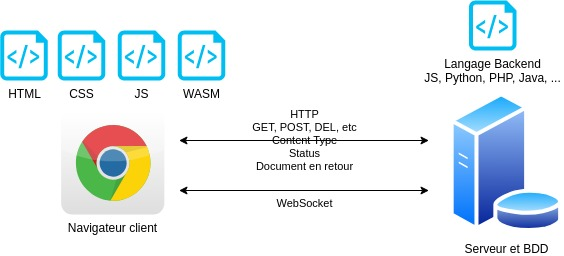
\includegraphics[width=11cm]{image/web-stakeholders.drawio}
    \end{frame}


    \section{Le web statique}\label{sec:static}

    \begin{frame}{Le web statique}
        Une des premières options pour un site web est donc d'être statique.

        Suite à une requête sur une URL (adresse dans le navigateur), le serveur nous envoie une page HTML pour la donnée avec du CSS pour le style.
        \bigbreak
        Il n'y a pas d'interaction avec le serveur, le contenu est figé, on peut juste passer à une autre page grâce à une ancre \lstinline{<a href="...">...</a>}.
        \bigbreak
        \centering
        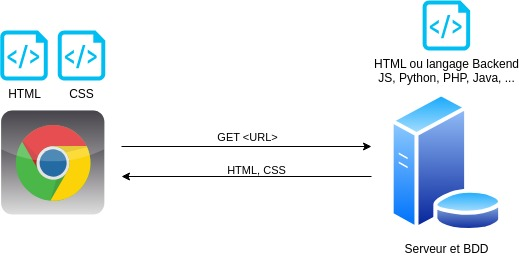
\includegraphics[width=8cm]{image/web-static}
    \end{frame}

    \begin{frame}[fragile]{Développement Web Statique}{Exercice \execcounterdispinc{}}
        \begin{itemize}
            \item Installer Python 3.
            \item Installer un IDE de développement Web comme WebStorm.
            \item Lancer un serveur HTTP avec la commande dans le répertoire du cours~:
            \begin{lstlisting}[language=bash]
python3 -m http.server
            \end{lstlisting}
            \item Naviguer à l'adresse indiquée.
            \item Modifier le fichier \lstinline{index.html} pour ajouter un lien vers une page HTML développée par vos soins avec votre nom et une photo de vous.
            \item Rafraîchir la page et vérifier que la modification est fonctionnelle.
        \end{itemize}
    \end{frame}


    \section{Le web dynamique}\label{sec:Dynamic}
    \begin{frame}{Développement Web Dynamique}{Exercice \execcounterdispinc{}}
        \begin{itemize}
            \item Quelles seraient les moyens d'avoir des pages web dynamiques~?
        \end{itemize}
        \bigbreak
        \centering
        
\includegraphics[width=5cm]{image/question-mark}
    \end{frame}

    \begin{frame}{Développement Web Dynamique}{Backend}
        Un serveur qui fait tourner un algorithme qui sert des données qui évoluent (dans la base de données), ou de l'extérieur (API).

        Plusieurs requêtes sont nécessaires, de différents types~:
        \begin{itemize}
            \item Des GET comme auparavant pour retourner des données.
            \item Des POST pour envoyer des données au serveur.
            \item Des DEL pour supprimer des données de la base de données du serveur.
        \end{itemize}
        \bigbreak
        \centering
        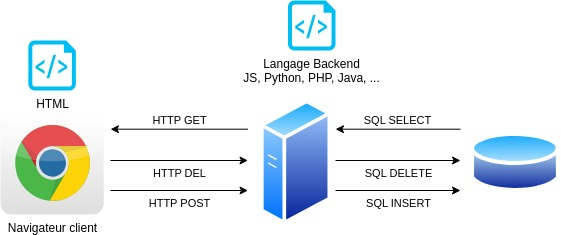
\includegraphics[width=7cm]{image/web-dynamic-backend}
    \end{frame}

    \begin{frame}{Frontend}
        \begin{small}
            Il est également possible de modifier une page web sans recharger la page entière, en utilisant JavaScript.

            Le JavaScript est un des langages qui peut être interprétés par le navigateur.

            Ces langages sont~:
            \begin{itemize}
                \item \textbf{HTML}, un langage de balisage, à l'image du XML, c'est le document principal de la page.
                Il peut contenir de la mise en forme, des données à afficher, \textit{etc}.
                \item \textbf{CSS}, un langage de style, qui permet de définir la mise en forme de la page.
                C'est une manière \textbf{modulaire} de définir le style de tout un site web.
                \item \textbf{JavaScript}, un langage de programmation qui permet de modifier le contenu de la page sans recharger la page.
                Il peut modifier~:
                \begin{itemize}
                    \item Le contenu de la page, ses données (DOM API\footnotemark{}).
                    \item Le style de la page, la mise en forme (DOM API\cref{DOM}).
                    \item Intéragir avec n'importe quel serveur.
                \end{itemize}
            \end{itemize}
        \end{small}
        \footnotetext{\label{DOM}DOM (Document Object Model), \url{https://developer.mozilla.org/fr/docs/Glossary/DOM}}
    \end{frame}


    \section{Généralité sur le JavaScript en Frontend}\label{sec:js-basic}

    \subsection{Où est-il~?}\label{sec:where}

    \begin{frame}{Où se trouve le JavaScript ?}
        Deux solutions, ils se trouvent~:
        \begin{itemize}
            \item Dans le fichier HTML, entre les balises \lstinline{<script>...</script>}.
            \item Dans un fichier séparé, avec l'attribut \lstinline{src} de la balise \lstinline{<script>} qui indique le chemin de ce fichier.
            Comme le fichier de style, cette méthode est plus modulaire, car ce fichier peut être partagé entre plusieurs pages.
        \end{itemize}
        \bigbreak
        \begin{dangercolorbox}
            En programmation, être modulaire est une qualité importante. Si on réutilise, on est écrit moins.
            Ici, dans un seul fichier.
            Si on écrit moins, on écrit moins de bug~!
        \end{dangercolorbox}
    \end{frame}

    \begin{frame}{Exercice \execcounterdispinc{}}
        \begin{itemize}
            \item Trouver le script javascript du fichier \lstinline{index.html}.
            \item Créer un fichier \lstinline{script.js} dans le même répertoire que \lstinline{index.html}.
            \item Copier le contenu du script dans ce fichier.
            \item Adapter le fichier \lstinline{index.html} pour inclure ce fichier en utilisant l'attribut \lstinline{src} et supprimant le contenu de la balise qui devient inutile.
            \item Simplifier la balise \lstinline{<script>} en conséquence.
            \item Rafraîchir la page et vérifier que la modification est fonctionnelle, \textit{i.e.}, que le contenu est le même.
            \item Créer une autre page HTML qui appelle ce même script.
            \item Vérifier que cette dernière affiche le dernier paragraphe indiquant le temps.
        \end{itemize}
        Comprenez-vous l'aspect \textit{modulaire} de cette méthode~?
    \end{frame}

    \subsection{Les bases du débug}\label{sec:debugbasics}
    \begin{frame}{Les bases du débug}{Dans le navigateur}
        Le JavaScript est exécuté par le navigateur, il est donc essentiel de pouvoir débugger ce dernier directement dans le navigateur.
        \bigbreak
        On peut y inspecter~:
        \begin{itemize}
            \item Les éléments de la page, les balises HTML.
            \item Les requêtes HTTP, c’est-à-dire, le traffic réseau.
            \item Les erreurs JavaScript.
            \item Modifier le code HTML, JS, CSS de la page en direct.
            \item Analyser l'usage des ressources mémoire (RAM) et stockage de données.
            \item Le responsive design avec un simulateur de mobile/tablette.
            \item \textit{many more}.
        \end{itemize}
        Ils sont accessibles avec la touche \lstinline{F12}.
    \end{frame}

    \begin{frame}{Les bases du débug}{Inspection du HTML}
        2 solutions~:
        \begin{itemize}
            \item Clic droit sur un élément de la page, puis \textit{Inspecter}.
            \item Avec F12 dans l'\textit{inspecteur}, naviguer dans l'arborescence des balises HTML et observer la page.
            Les éléments sont mis en surbrillance lorsqu'on survole les balises correspondantes.
        \end{itemize}
        \bigbreak
        \centering
        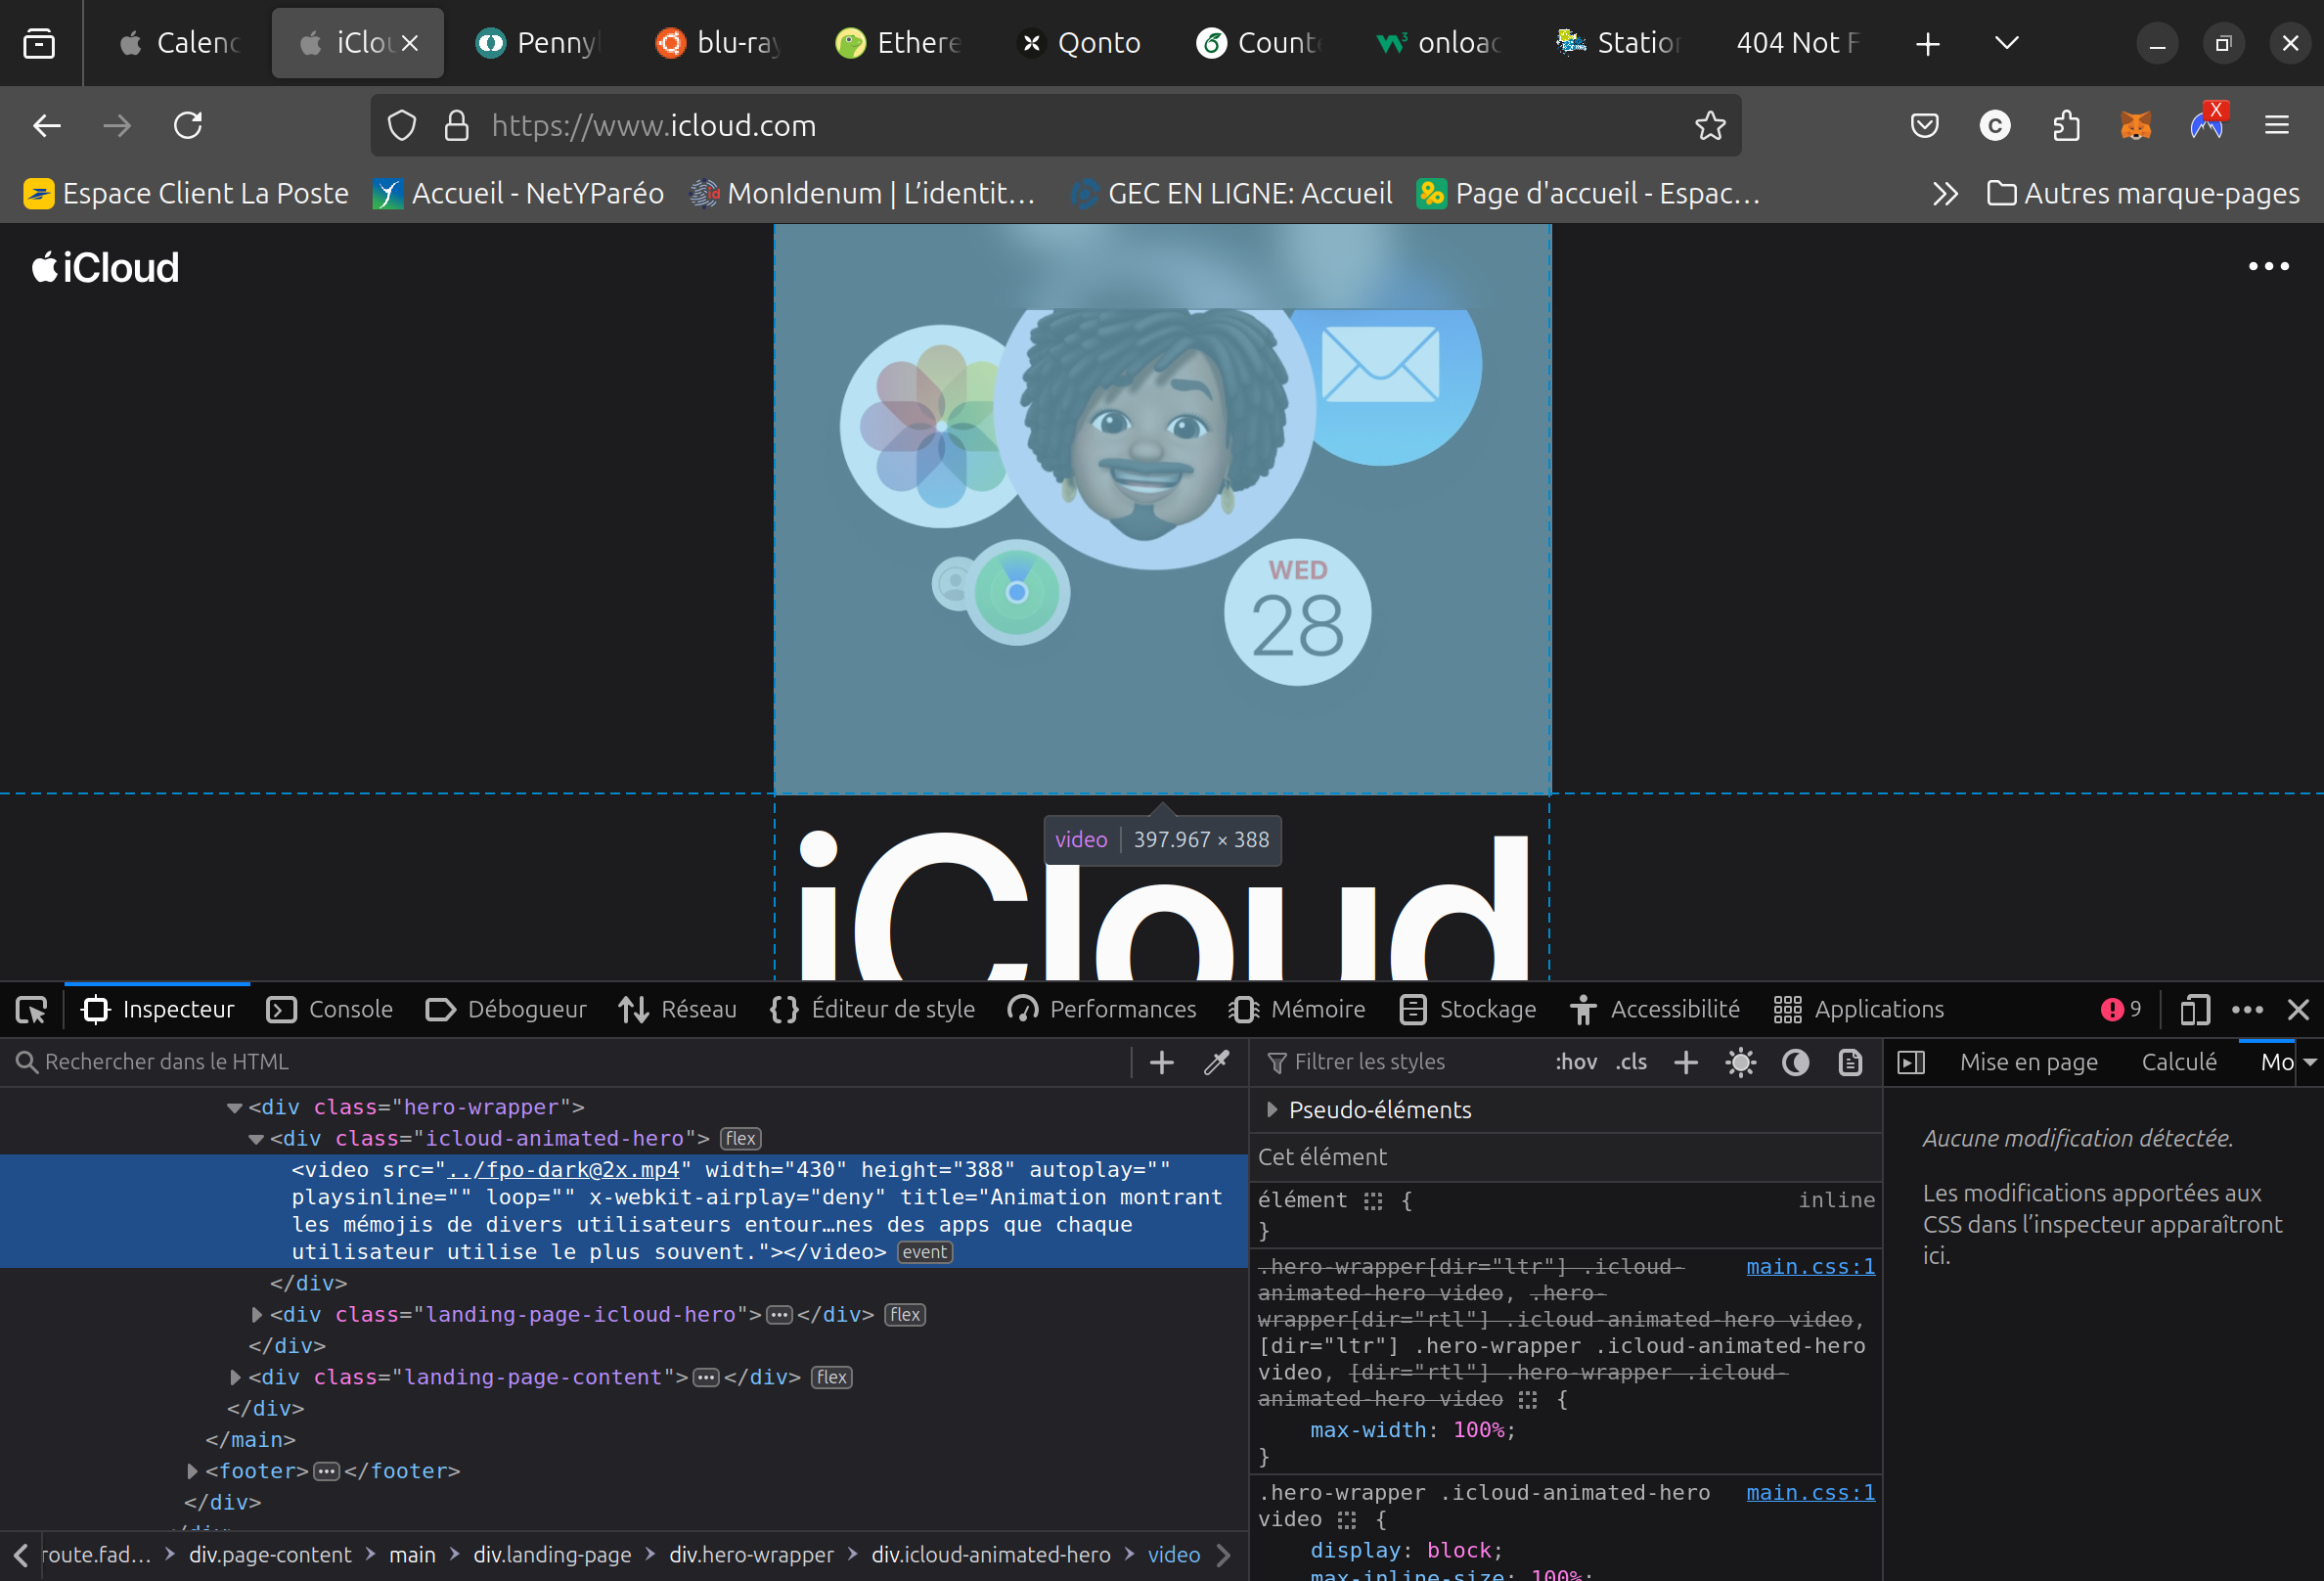
\includegraphics[width=7cm]{image/inspector-highlight}
    \end{frame}

    \begin{frame}{Les bases du débug}{Inspection du HTML}
        Exercice \execcounterdispinc{}~:
        \bigbreak
        \begin{itemize}
            \item Inspecter la page \url{https://www.icloud.com/calendar/}.
            \item Trouver la classe du texte \textit{Organisez votre temps avec Calendrier iCloud. Vos calendriers sont toujours à jour sur n’importe quel appareil et sur le Web.}.
            \item Trouver la police de caractère de cette classe.
            \item Modifier la police de caractère de cette classe pour \textit{Comic Sans MS} et vérifier la prise en compte de la modification.
        \end{itemize}
        \bigbreak
        \centering
        
\includegraphics[width=3cm]{image/intelligence}
    \end{frame}

    \begin{frame}{Les bases du débug}{La console}
        La console est dédiée au JS, elle permet d'écrire du JS ou d'appeler du JS déjà connu de la page.
        \bigbreak
        \centering
        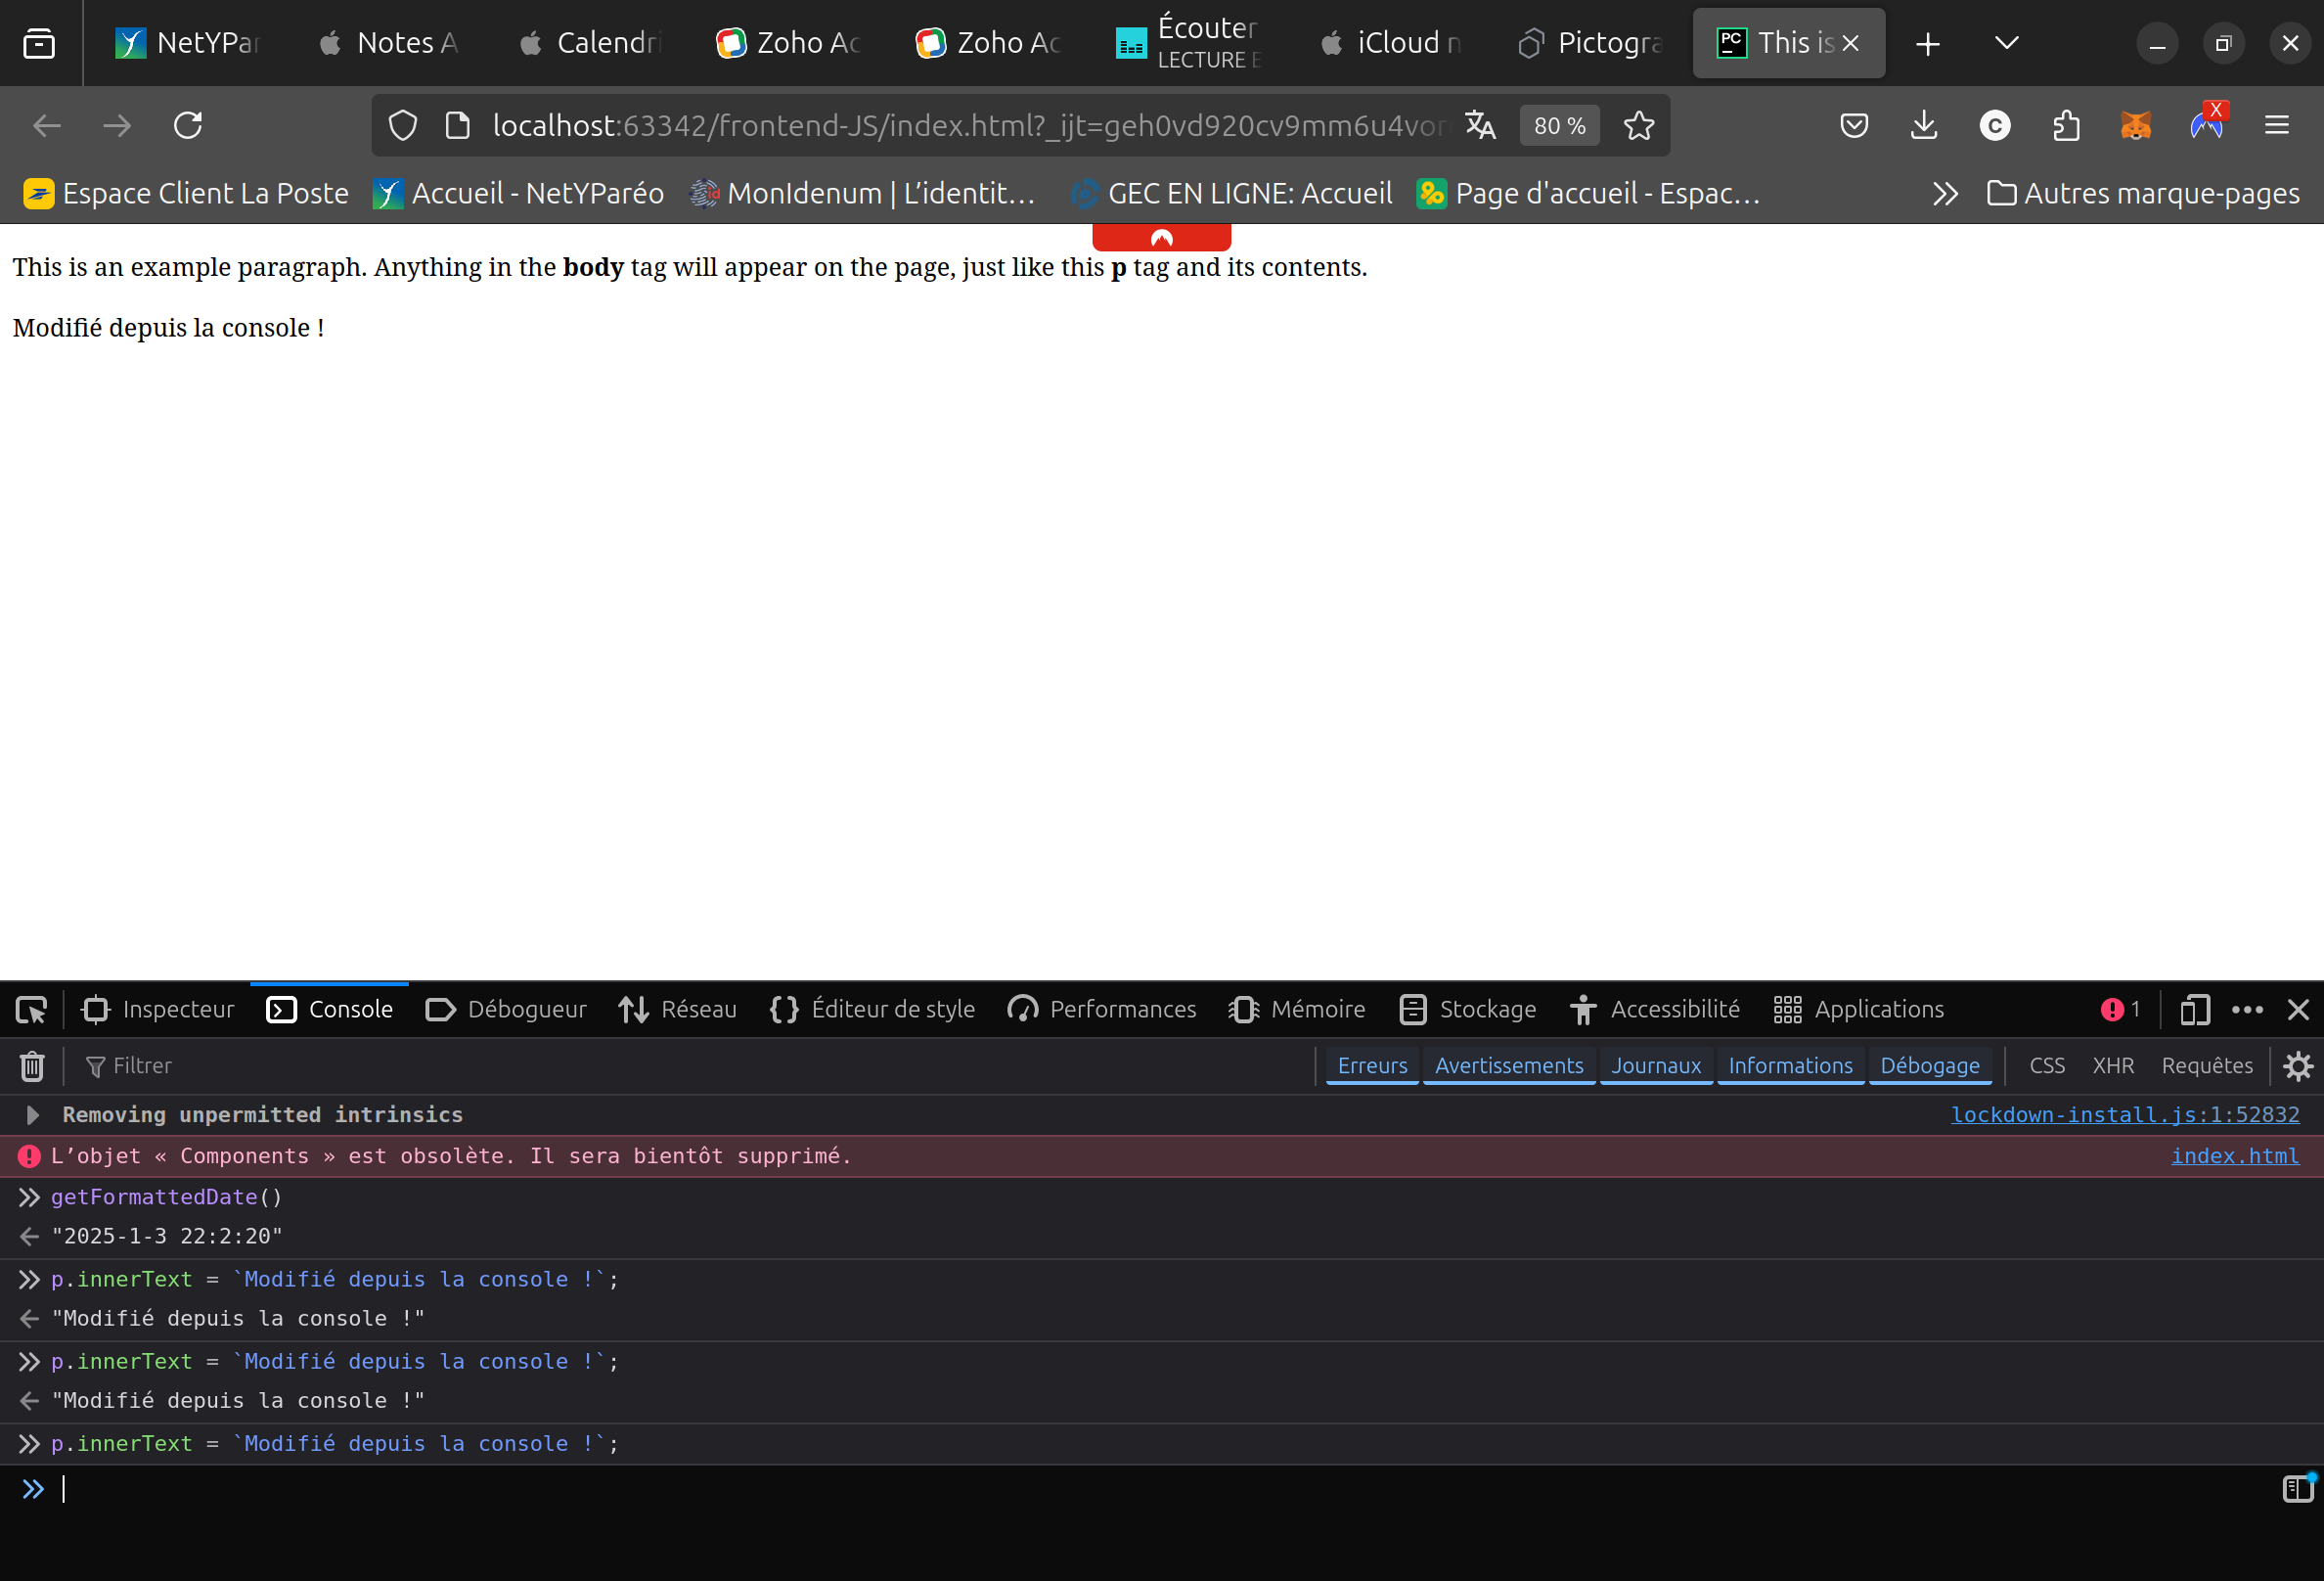
\includegraphics[width=8cm]{image/js-in-console}
        \bigbreak
        \flushleft
        Expliquer le comportement ci-dessus.
    \end{frame}

    \begin{frame}{Les bases du débug}{La console}
        Elle affiche (\textit{log}) les éventuels messages de warning, info, erreur lors de l'exécution et les erreurs de syntaxe.
        \bigbreak
        \centering
        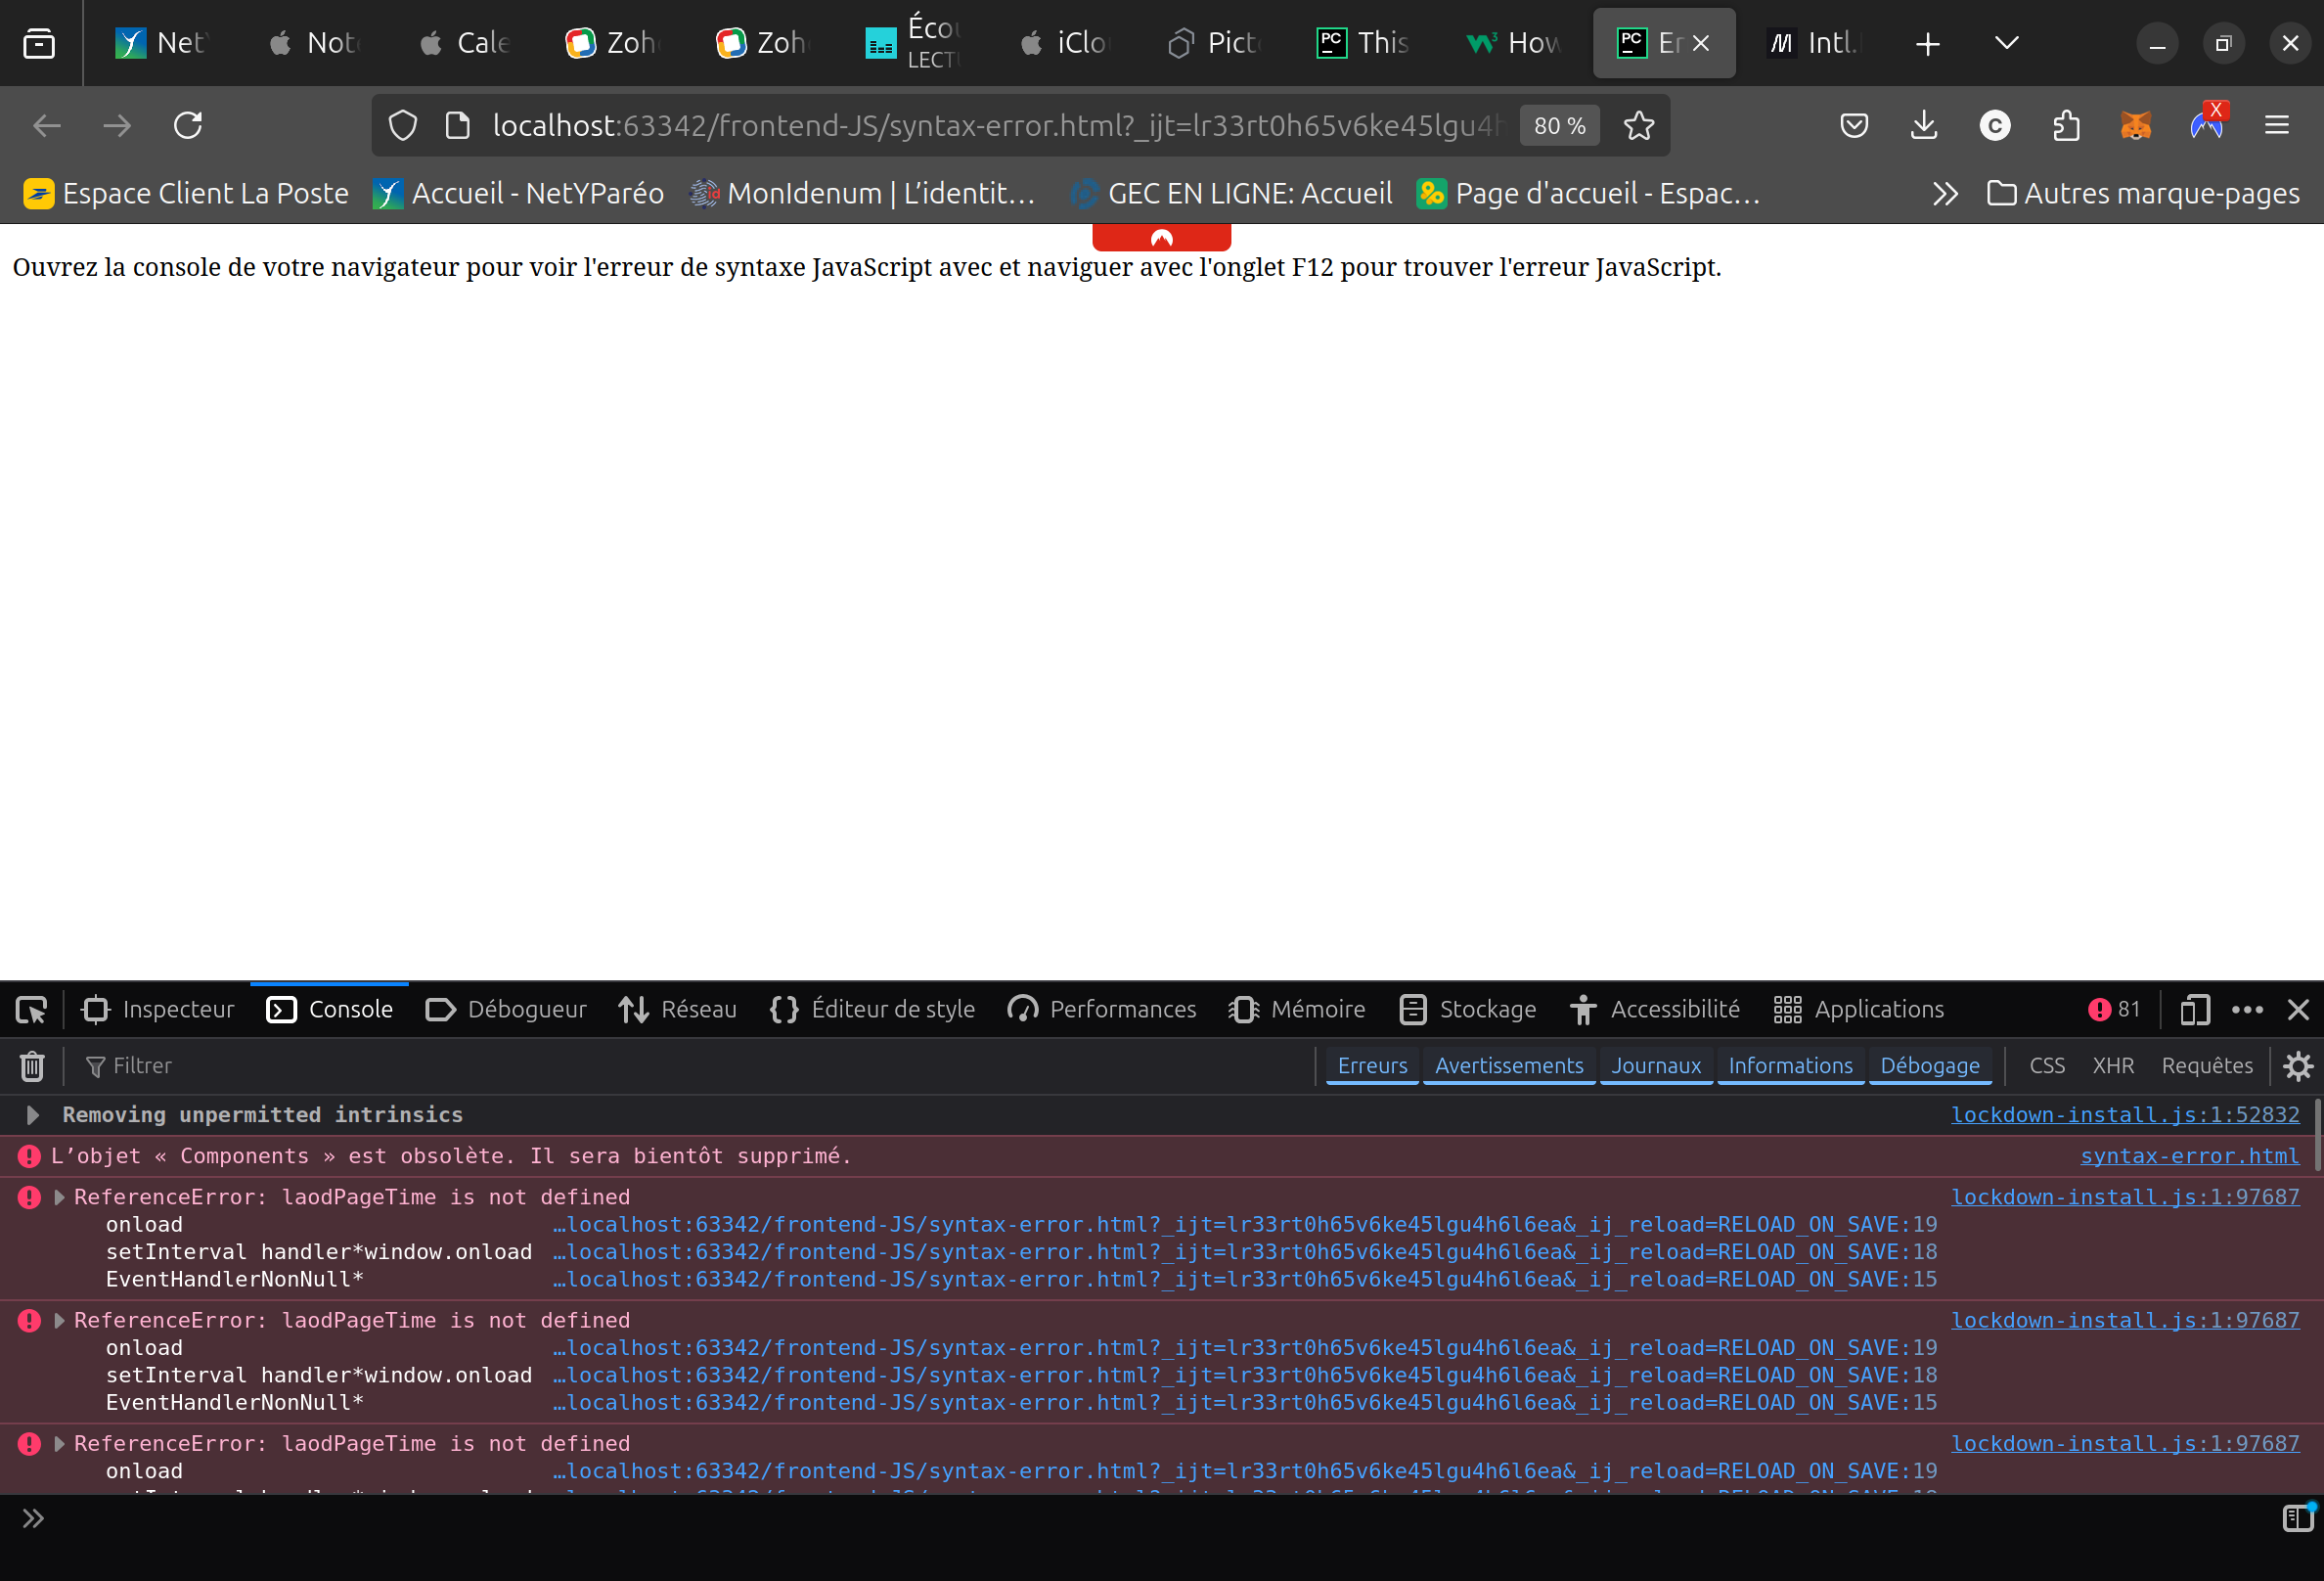
\includegraphics[width=7cm]{image/js-console-error-message}
        \flushleft
        On voit ici le parcours de l'interpréteur jusqu'à l'erreur en commençant par le dernier des appels.
    \end{frame}

    \begin{frame}{Les bases du débug}{La console}
        En cliquant sur le lien, on arrive sur le code source de l'erreur dans le débogueur.
        \bigbreak
        \centering
        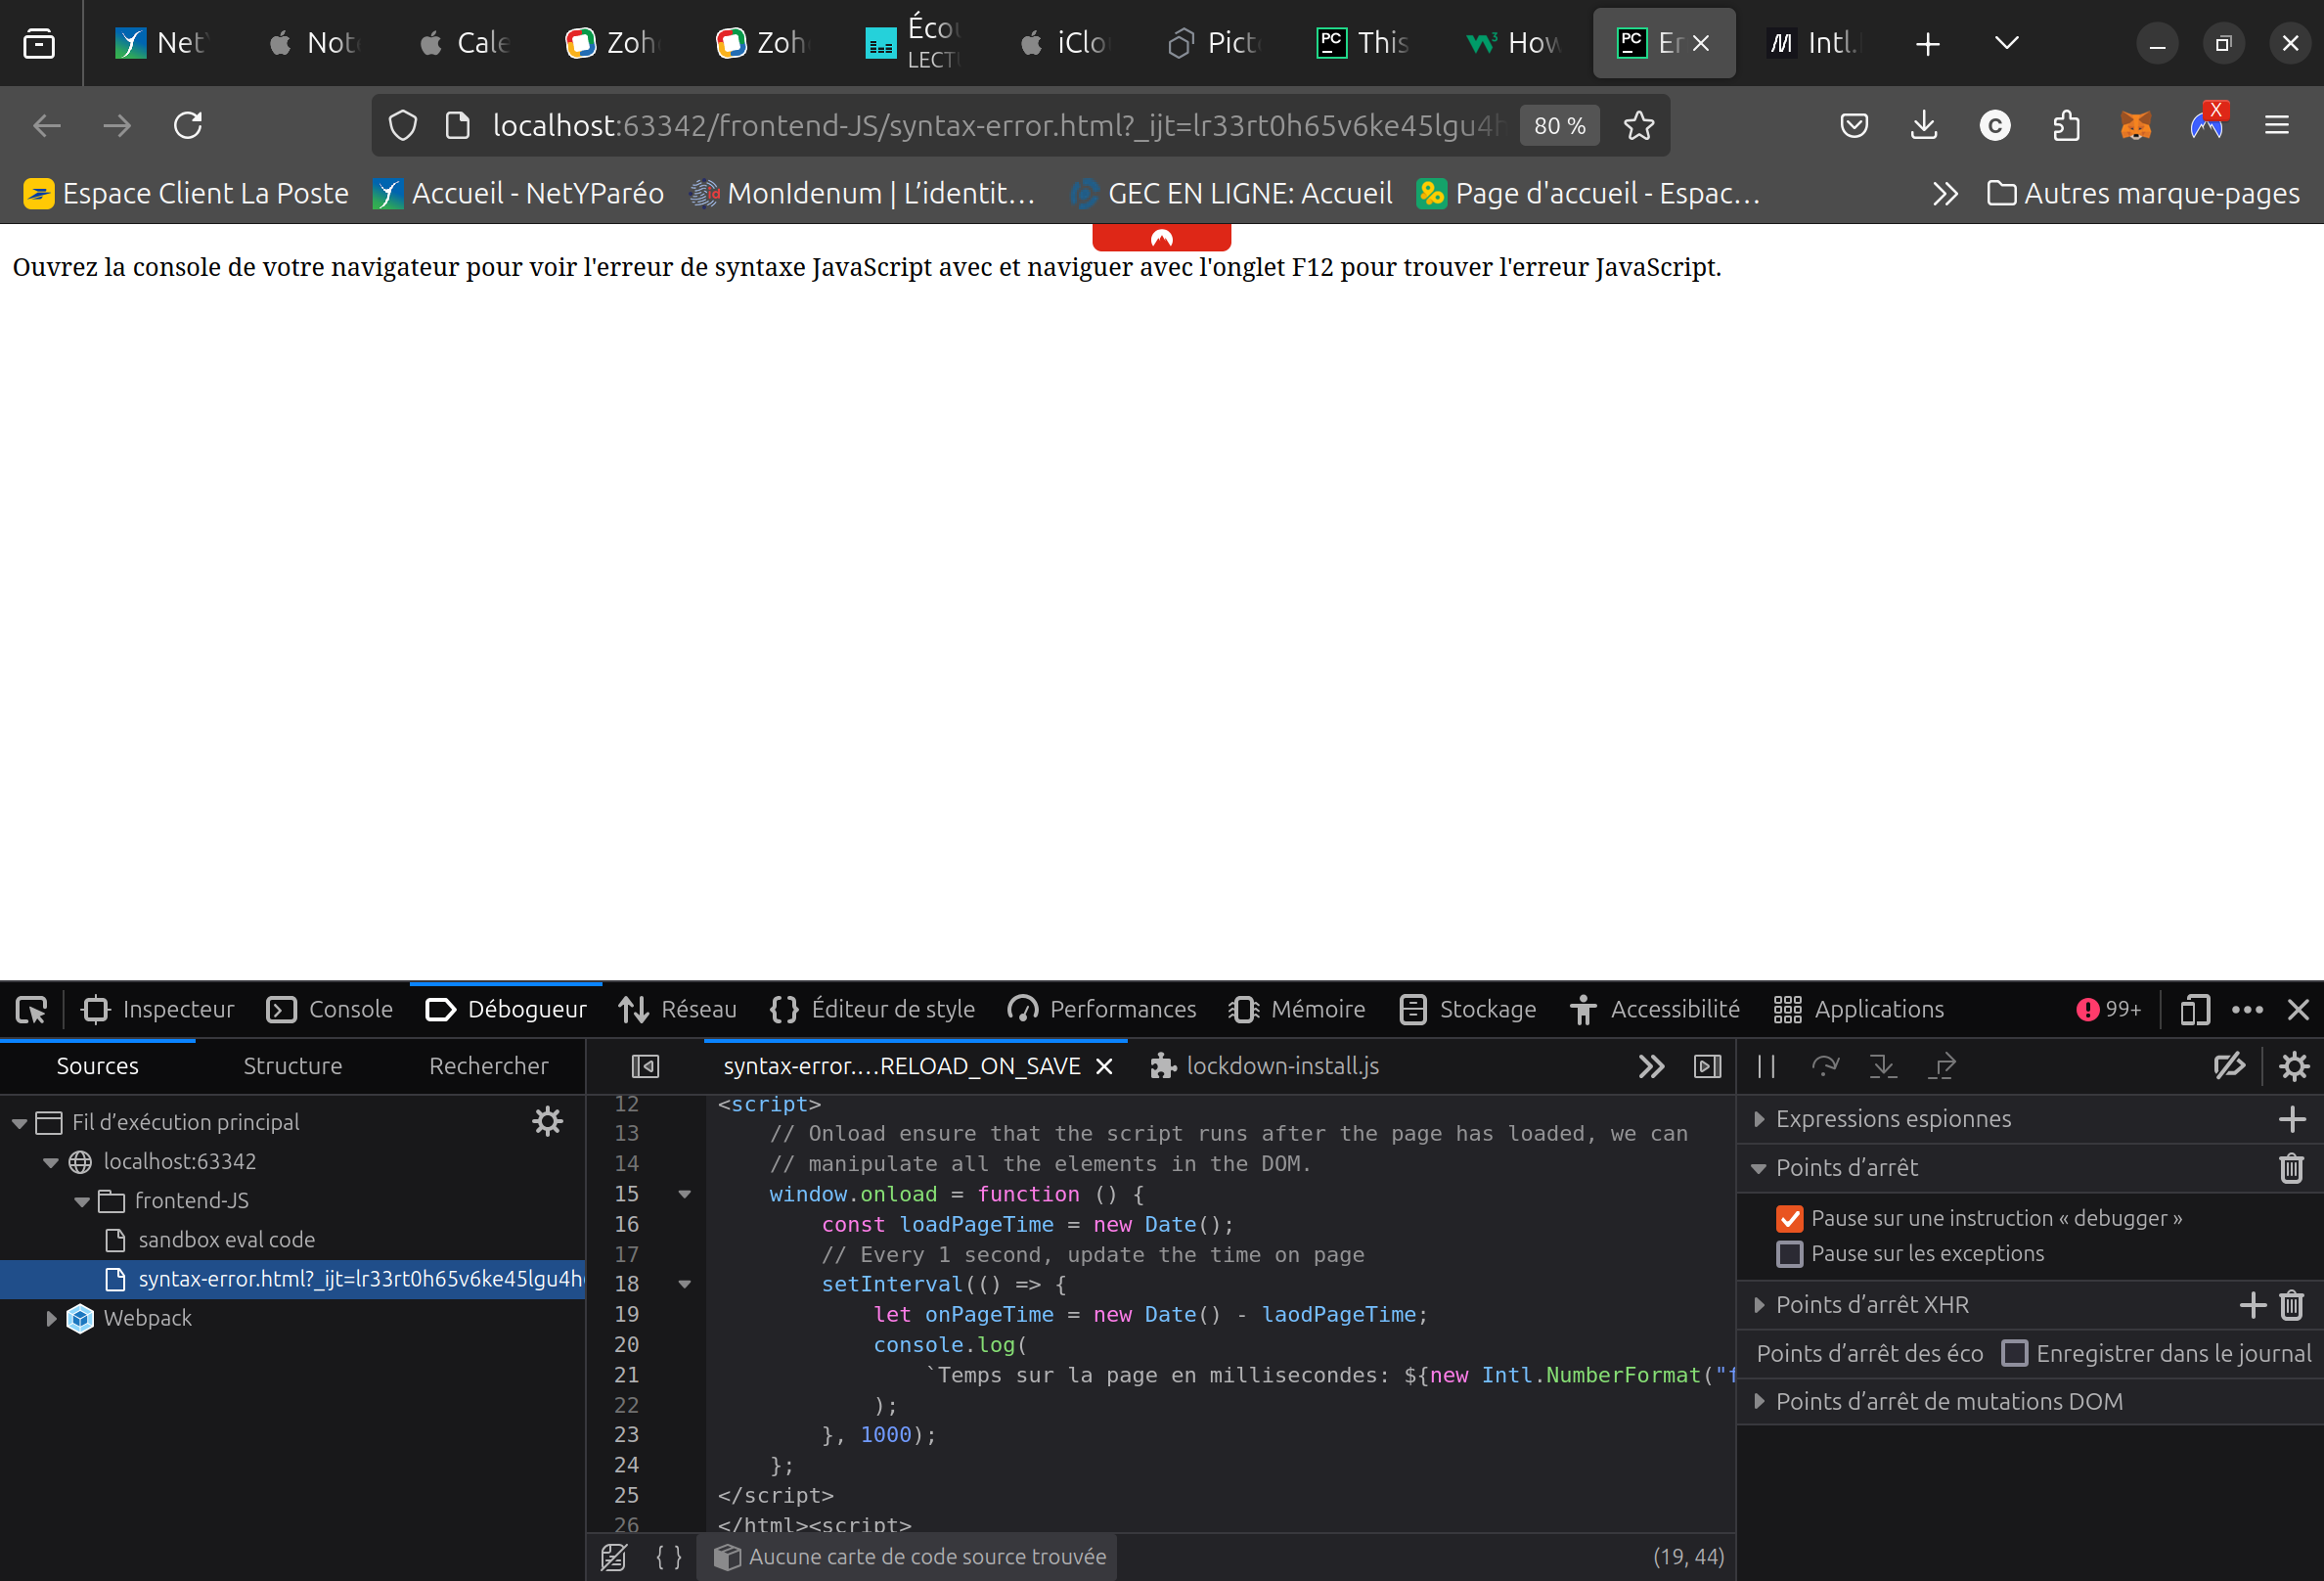
\includegraphics[width=9cm]{image/js-console-error-code}
    \end{frame}

    \begin{frame}{Les bases du débug}{Le débogueur}
        Le débogueur est, lui aussi, dédié au JS, il permet~:
        \begin{itemize}
            \item De lire le JS de la page.
            \item De mettre des points d'arrêt (\textit{breakpoints}) pour arrêter l'exécution du code.
            \item De naviguer dans le code, de pas en pas, de sauter des fonctions.
            \item De voir les valeurs des variables à un instant donné.
            \item De voir la pile d'appel des fonctions.
        \end{itemize}
    \end{frame}

    \begin{frame}{Les bases du débug}{Le débogueur}
        \bigbreak
        \centering
        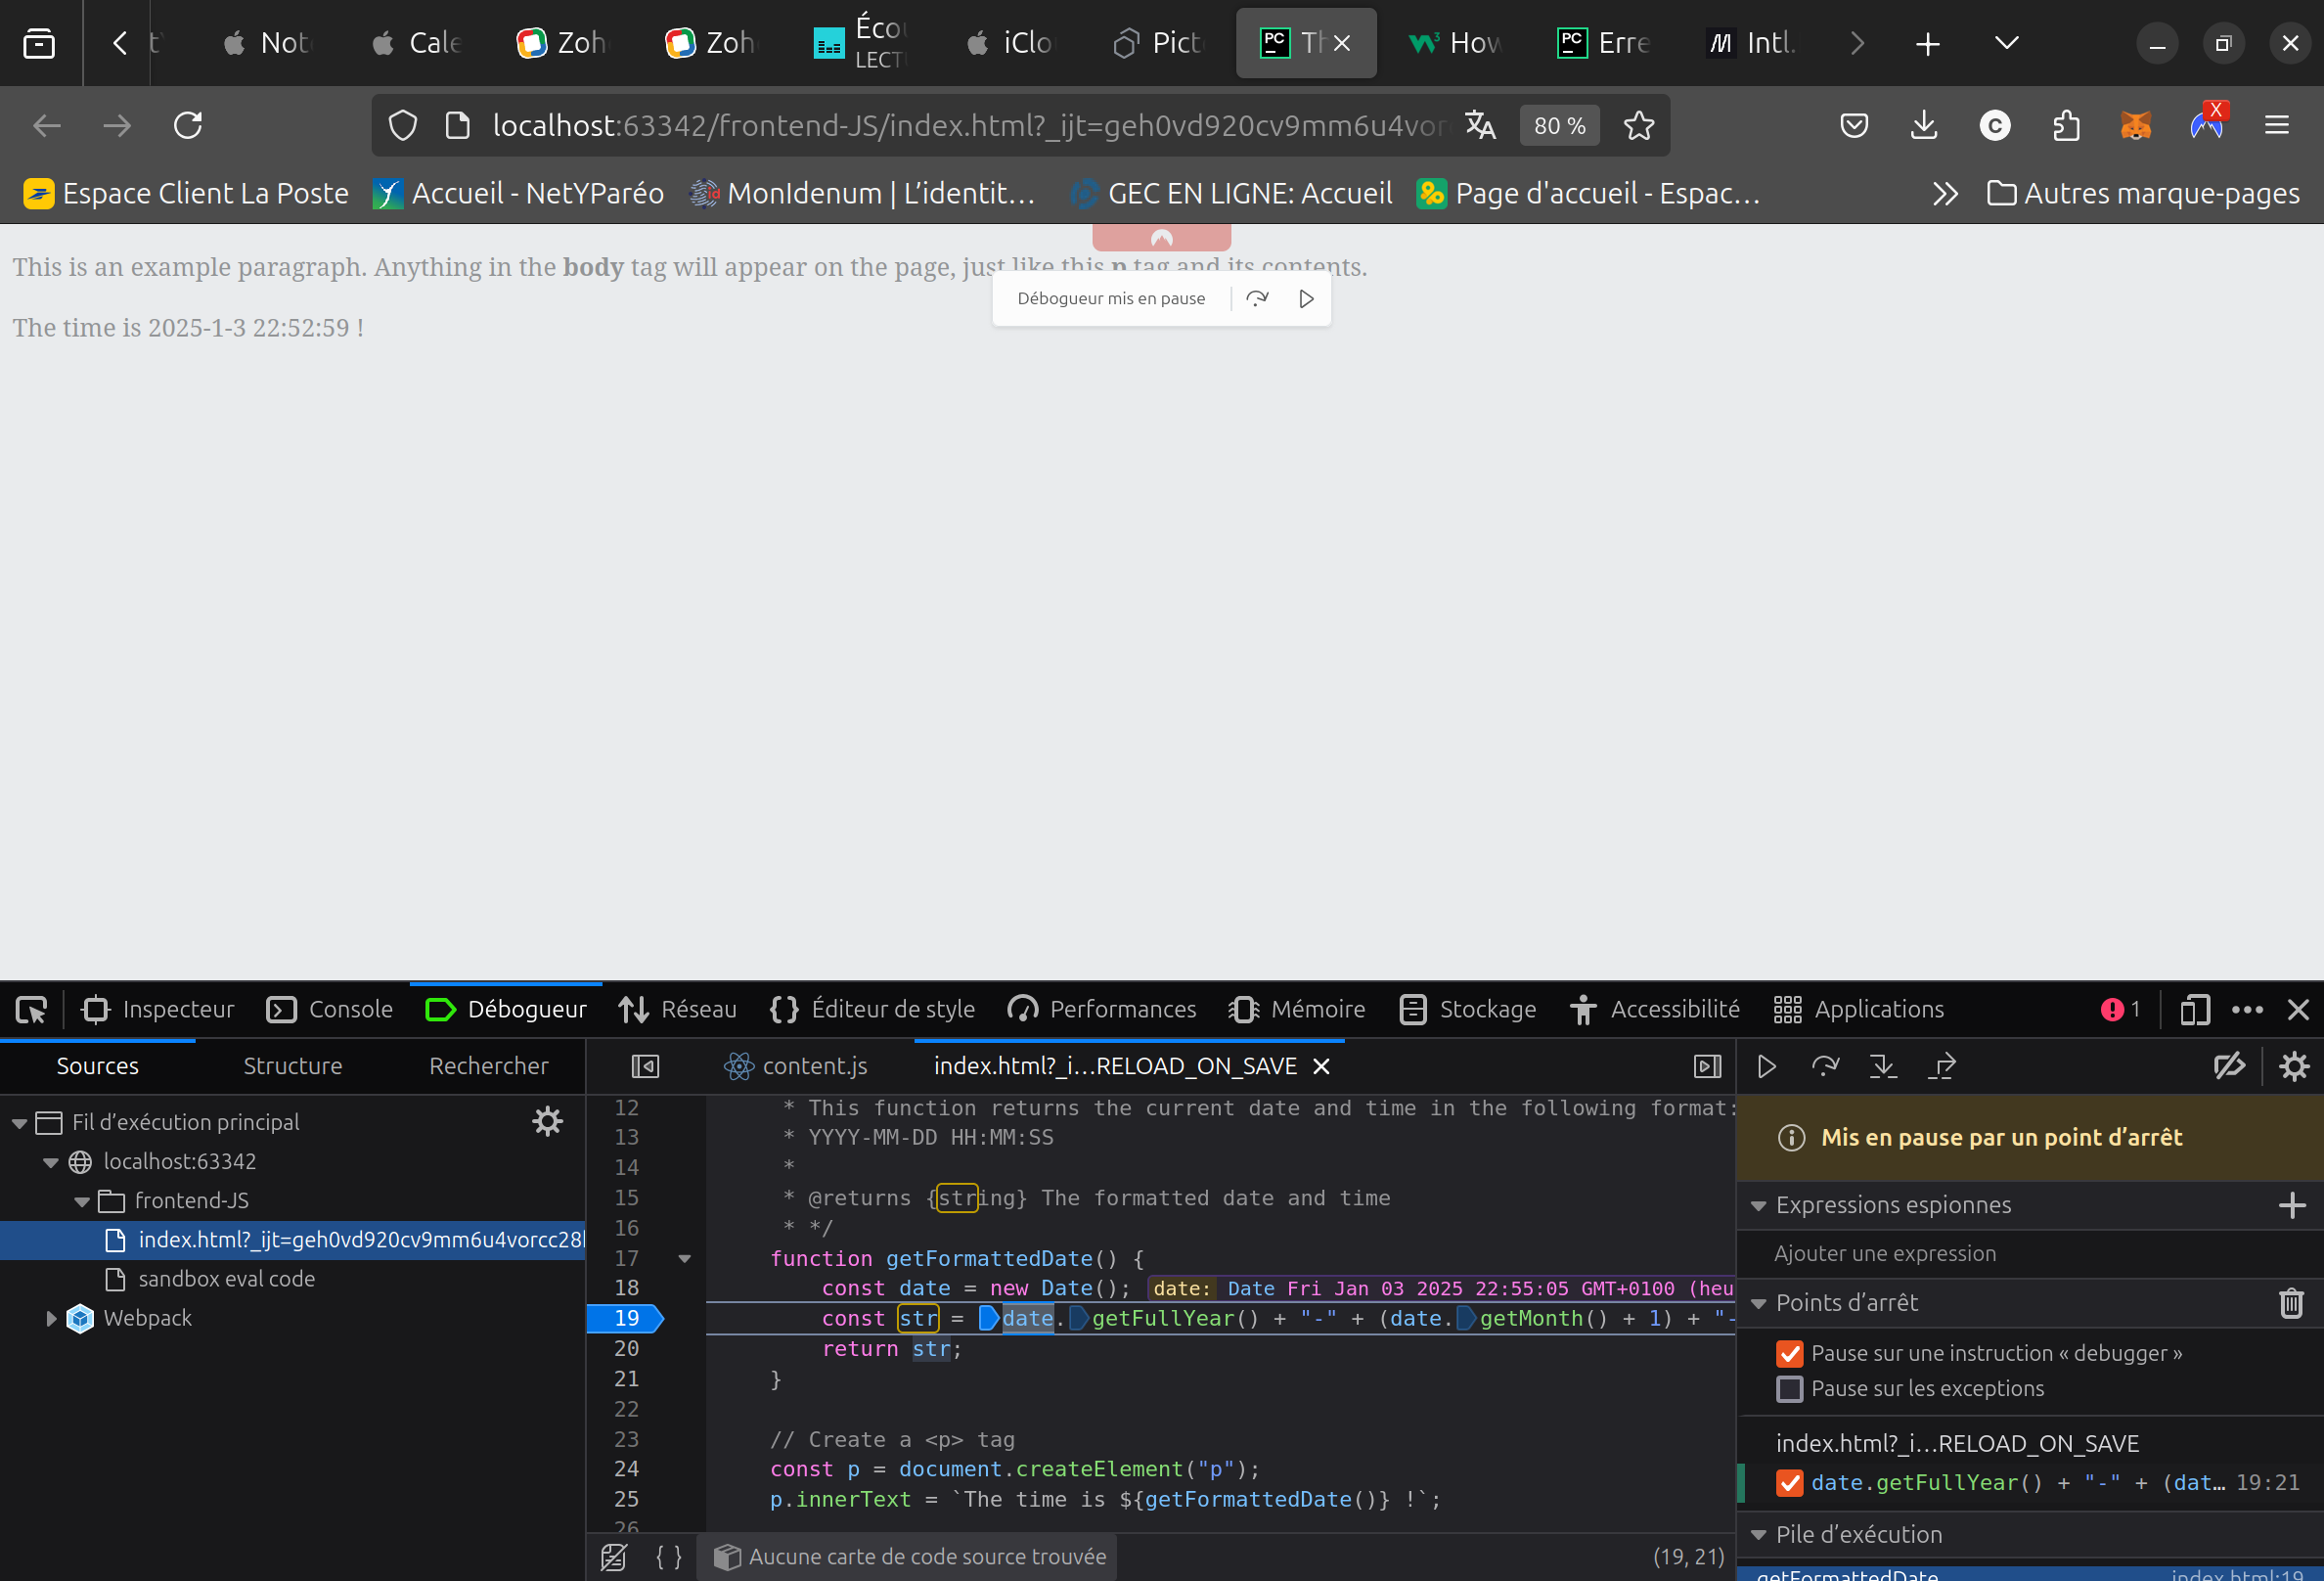
\includegraphics[width=10cm]{image/js-debugger}
    \end{frame}

    \begin{frame}{Les bases du débug}{Console et débogueur}
        Exercice \execcounterdispinc{}~:
        \begin{itemize}
            \item Naviguer à l'adresse \url{http://0.0.0.0/syntax-error.html}.
            \item Ouvrir la console.
            \item Cliquer sur le dernier appel pour aller au plantage
            \item Lire le code dans le débuggeur pour trouver l'erreur.
            \item Corriger l'erreur dans le code source et recharger la page.
        \end{itemize}
        \bigbreak
        \centering
        
\includegraphics[width=3cm]{image/intelligence}
    \end{frame}

    \begin{frame}{Les bases du débug}{Débogueur}
        Exercice \execcounterdispinc{}~:
        \begin{itemize}
            \item Naviguer à l'adresse \url{http://0.0.0.0/}.
            \item Ouvrir la débuggeur.
            \item Ajouter un point d'arrêt dans la fonction \lstinline{getFormattedDate}.
            \item Observer ce qui se passe.
            \item Faire du pas à pas pour comprendre le code.
        \end{itemize}
        \bigbreak
        \centering
        
\includegraphics[width=3cm]{image/intelligence}
    \end{frame}


    \section{Le langage JavaScript}\label{sec:js-lang}
    \begin{frame}{JavaScript}{L'historique\footnote{\label{mozilla-js}Une réintroduction à JavaScript, \url{https://developer.mozilla.org/fr/docs/Web/JavaScript/Language_overview}}}
        \begin{footnotesize}
            \begin{itemize}
                \item Créé en 1995 par Brendan Eich chez Netscape.
                \item En 1996, Java est très populaire et Netscape veut surfer sur la vague et renomme le langage appelé LiveScript en JavaScript.
                \item Standardisé par l'ECMA (European Computer Manufacturers Association) en 1997.
                \item Le standard est l'ECMAScript.
                \item La version actuelle implémentée dans les navigateurs se base sur le standard ES6 de 2015/2016.
                \item Les navigateurs implémentent des versions différentes de l'ES.
                \item JS est partout dans le backend ou programmation système avec Bun ou Node.js, pour le scripting de NoSQL comme CouchDB ou MongoDB, dans les PDF, \textit{etc}.
                \item Paradigme de programmation orienté objet mais s'adapte très bien au fonctionnel aussi et de mieux en mieux\ldots
            \end{itemize}
        \end{footnotesize}
    \end{frame}

    \begin{frame}{L'écosystème JavaScript}{Un langage interprété}
        \centering
        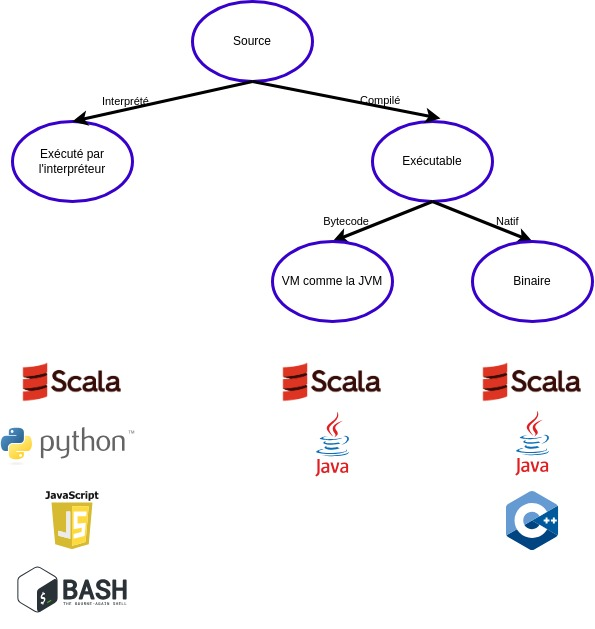
\includegraphics[width=7cm]{image/code-inter-vs-compiled}
    \end{frame}

    \begin{frame}{L'écosystème JavaScript}{Un langage interprété}
        \begin{small}
            De nombreux interpréteurs JavaScript existent dans les navigateurs, mais aussi en dehors~:
            \begin{itemize}
                \item \textbf{V8}, le moteur JavaScript de Chrome.
                \item \textbf{Node.js}, un interpréteur JavaScript côté serveur basé sur V8.
                \item \textbf{Deno}, un interpréteur JavaScript côté serveur basé sur V8, écrit en Rust par le développeur Node.js, il devrait lui succéder.
                \item \textbf{JavaScriptCore}, le moteur JavaScript de Safari.
                \item \textbf{SpiderMonkey}, le moteur JavaScript de Firefox.
                \item \textbf{Bun}, un environnement d'exécution plus rapide que Node.js et Deno\footnote{\label{bun}Bun is a fast JavaScript, \url{https://bun.sh/}}.
                \item \textbf{CouchDB}, une base de données NoSQL qui utilise JavaScript pour les requêtes dans sa version ES6 grâce à son binding avec SpiderMonkey, \footnote{The Road to CouchDB 3.0: Update to JavaScript Engine, \url{https://blog.couchdb.org/2020/02/26/the-road-to-couchdb-3-0-update-to-javascript-engine/}}.
                \item \textit{Many more}.
            \end{itemize}
        \end{small}
    \end{frame}

    \begin{frame}{L'écosystème JavaScript}{Les limites de notre cours}
        Sachant que ce cours s'appelle \textit{JavaScript Frontend}, dans quel(s) partie(s) de l'écosystème JavaScript allons-nous nous programmer~?
        \bigbreak
        \centering
        
\includegraphics[width=3cm]{image/intelligence}
        \pause
        \bigbreak
        \flushleft
        Nous allons programmer du JavaScript exécuté dans le navigateur, donc du JavaScript côté client.
    \end{frame}

    \begin{frame}{JavaScript dans le navigateur}{Les limites}
        Il existe de nombreuses limites à ce que peut faire le JavaScript dans le navigateur, principalement pour des raisons de sécurité~:
        \begin{itemize}
            \item Pas d'accès au système de fichiers, A.K.A. \textit{File System}, le disque dur.
            \item Capacités réseau limitées, seule une partie du protocole HTTP et le protocole WebSocket.
            Tout ce qui est protocole de bas niveau comme TCP, UDP, \textit{etc} est interdit.
            Il ne peut être que client, pas serveur.
            \item Le stockage de données se fait dans le navigateur, dans les cookies, le \textit{localStorage}, le \textit{sessionStorage} principalement.
            \item Pas d'accès à l'OS, donc pas de gestion de processus, tout est isolé dans le navigateur.
        \end{itemize}
    \end{frame}

    \begin{frame}{JavaScript dans le navigateur}{Les spécificités}
        \begin{scriptsize}
            Les spécificités du navigateur sont ses 2 A.P.I. (Application Programming Interface)~:
            \begin{itemize}
                \item Le DOM (Document Object Model)\footnote{Référence du DOM, \url{https://developer.mozilla.org/fr/docs/Web/API/Document_Object_Model}}, qui permet de manipuler le contenu de la page dans les langages de balises HTML, XML, SVG.
                \item Le BOM (Browser Object Model)\footnote{Introduction au Browser Object Model (BOM) et à l’objet Window, \url{https://www.pierre-giraud.com/javascript-apprendre-coder-cours/browser-object-model-window/\#google_vignette}}, qui permet de manipuler le navigateur et ses fenêtres (\lstinline{window})~:
                \begin{itemize}
                    \begin{scriptsize}
                        \item L’objet \lstinline{Navigator} qui représente l’état et l’identité du navigateur et qu’on va utiliser avec l’API Geolocation.
                        \item L’objet \lstinline{History} qui permet de manipuler l’historique de navigation du navigateur.
                        \item L’objet \lstinline{Location} qui fournit des informations relatives à l’URL de la page courante.
                        \item L’objet \lstinline{Screen} qui nous permet d’examiner les propriétés de l’écran qui affiche la fenêtre courante.
                        \item L’objet \lstinline{Document} et le DOM dans son ensemble que nous étudierons en détail dans la suite.
                    \end{scriptsize}
                \end{itemize}
            \end{itemize}
        \end{scriptsize}
    \end{frame}

    \begin{frame}{JavaScript dans le navigateur\footnote{\label{eloquent-javaScript}Eloquent JavaScript, Marjin Haverbeke, \url{https://eloquentjavascript.net}}}{Les prérequis}
        Pour utiliser une API, quelle qu'elle soit, quel que soit le langage, il faut d'abord maîtriser les bases de ce dernier.
        \bigbreak
        Les bases de JS que nous allons couvrir ici sont les suivantes~:
        \begin{itemize}
            \item Les types
            \item La déclaration de variables
            \item Le scope des variables
            \item Les structures de contrôle (\textit{control flow})
            \item La déclaration de fonctions
            \item Les objets
            \item Les méthodes built-in
            \item Les exceptions
        \end{itemize}
    \end{frame}

    \subsection{Installation de WebStorm}\label{subsec:installwebstorm}

    \begin{frame}{Développement d'un script}{Installation d'un IDE}
        \begin{small}
            Un IDE est un \textit{Integrated Development Environment}, un environnement de développement intégré, logiciel d'édition de texte dédié à la programmation.
            \bigbreak
            Les principaux environnements de développement en JS sont VS Code de Microsoft et WebStorm de JetBrains.

            WebStorm est gratuit pour les étudiants, vous pouvez avoir une licence en créant un compte avec votre adresse MDS~.
            \bigbreak
            Installer également Node.js pour avoir un REPL (Read, Evaluate, Print and Loop)
        \end{small}
        \bigbreak
        \centering
        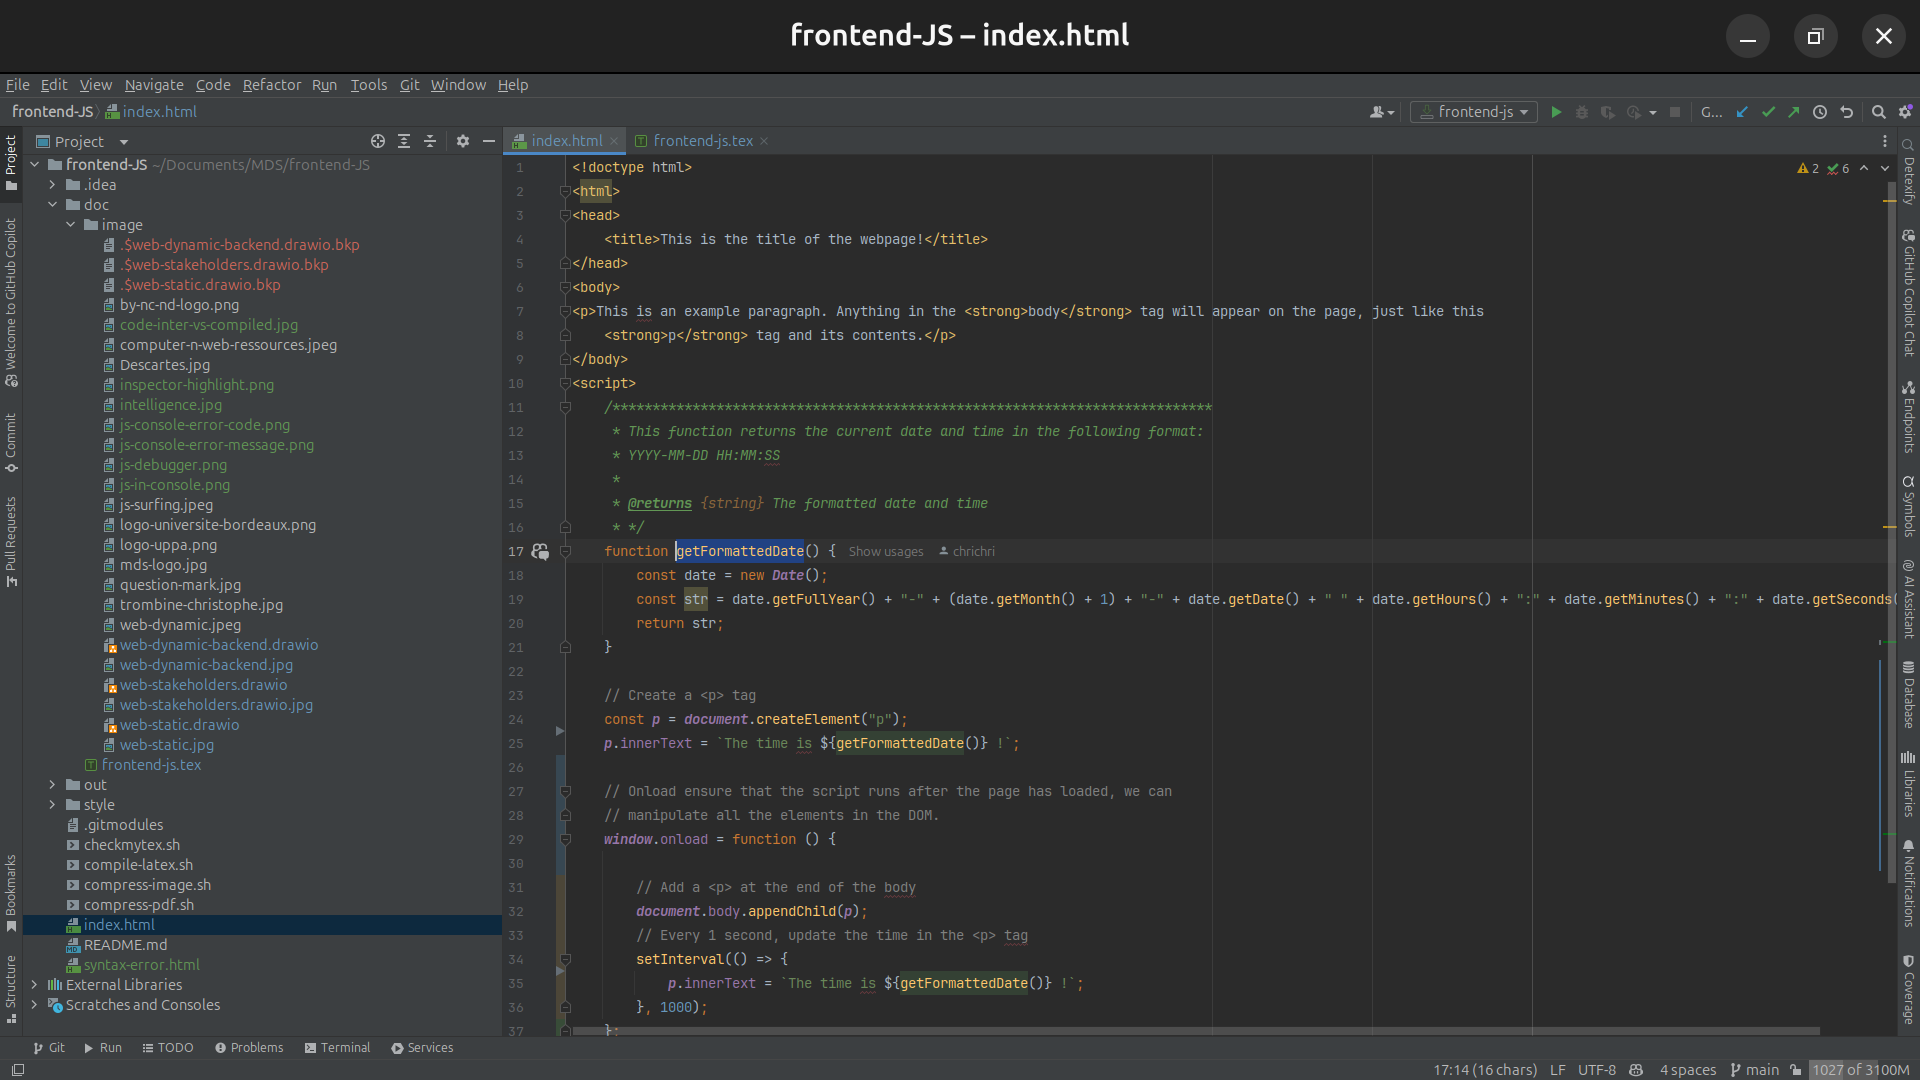
\includegraphics[width=6cm]{image/webstorm}
    \end{frame}

    \subsection{Initialisation du projet}\label{subsec:projectinit}

    \begin{frame}{Développement d'un script}{Mon premier script}
        \begin{itemize}
            \item Télécharger le code de ce cours sur GitHub \url{https://github.com/My-Digital-School-by-PapIT/frontend-JS}.
            \item Dézipper l'archive.
            \item Ouvrir le dossier avec WebStorm.
            \item Créer un fichier avec une extension comme \lstinline{variables-n-types.js} par exemple.
        \end{itemize}
        \bigbreak
        \centering
        
\includegraphics[width=3cm]{image/intelligence}
    \end{frame}

    \subsection{Déclarations et types primitifs}\label{subsec:declare-n-types}

    \begin{frame}[fragile]{Déclarations et types}{Les types numériques}
        \begin{lstlisting}[language=JavaScript,basicstyle=\tiny\ttfamily]
// Ceci est un commentaire et ne sera pas exécuté
/*
    Ceci est un commentaire multiligne et ne sera pas exécuté
 */

/*
Déclaration de variable numérique, elle a un scope avec var, un nom myAge et une
valeur à 39 dont le type est "inféré" par le langage, ici un type Number.
Toutes les déclarations se terminent par un ; par convention, il est optionnel.
 */
var myAge = 39; // 39 est un nombre entier (integer en anglais)
// Console.log est une fonction qui permet d'afficher des messages dans la console
console.log("J'ai " + myAge + " ans");
// Affiche le type de la variable myAge que l'on récupère avec l'opérateur typeof
console.log("Le type de la variable myAge qui n'a été déclaré (le type) est " + typeof myAge);

var myHeight = 1.85; // 1.75 est un nombre réel (float en anglais)
console.log("Je mesure " + myHeight + " mètre");
console.log("Le type de la variable myHeight qui n'a été déclaré (le type) est " + typeof myHeight);
// Les deux nombres entiers et réels sont de type Number en JavaScript.

// Mais peut aussi être déclaré de manière explicite
var myAge = Number(39); // 39 est un nombre entier (integer en anglais)
// Console.log est une fonction qui permet d'afficher des messages dans la console
console.log("J'ai " + myAge + " ans");
// Affiche le type de la variable myAge que l'on récupère avec l'opérateur typeof
console.log("Le type de la variable myAge qui n'a été déclaré (le type) est " + typeof myAge);
var myHeight = Number(1.85); // 1.75 est un nombre réel (float en anglais)
console.log("Je mesure " + myHeight + " mètre");
console.log("Le type de la variable myHeight qui n'a été déclaré (le type) est " + typeof myHeight);
        \end{lstlisting}
    \end{frame}

    \begin{frame}[fragile]{Déclarations et types}{Les grands entiers}
        \begin{lstlisting}[language=JavaScript]
/* Mais pour l'arithmétique des grands nombres, il est préférable d'utiliser BigInt.
    Ils sont à utiliser au-dessus du nombre définit dans Number.MAX_SAFE_INTEGER
    qui peut varier en fonction des machines
 */
console.log("Le nombre maximum de Number est " + Number.MAX_SAFE_INTEGER);
var myBigNumber = BigInt(Number.MAX_SAFE_INTEGER) + BigInt(1);
console.log("Le type de la variable myBigNumber qui n'a été déclaré (le type) est " + typeof myBigNumber);
        \end{lstlisting}
        \begin{dangercolorbox}
            Mais BigInt ne fonctionne que pour les entiers, pas les réels.
        \end{dangercolorbox}
        \begin{lstlisting}[language=Bash]
> var myBigNumber = BigInt(Number.MAX_SAFE_INTEGER) + BigInt(1.666);
Uncaught:
RangeError: The number 1.666 cannot be converted to a BigInt because it is not an integer
    at BigInt (<anonymous>)
> var myBigNumber = BigInt(Number.MAX_SAFE_INTEGER) + 1.666;
Uncaught TypeError: Cannot mix BigInt and other types, use explicit conversions
        \end{lstlisting}
    \end{frame}

    \begin{frame}[fragile]{Déclarations et types}{Les nombres speciaux}
        Un nombre particulier existe en JS c'est \textit{Infinity} qui représente l'infini.
        \begin{lstlisting}[language=JavaScript]
// Le nombre spécial Infinty
console.log("Le type de la variable Infinity qui n'a été déclaré (le type) est " + typeof Infinity);
console.log("Infinity - Infinity = " + Infinity - Infinity);
console.log("Infinity / 999999999999999999 = " + Infinity / 999999999999999999);
console.log("999999999999999999 / Infinity = " + 999999999999999999 / Infinity);
        \end{lstlisting}
    \end{frame}

    \begin{frame}[fragile]{Déclarations et types}{Les chaines de caractères}
        \begin{lstlisting}[language=JavaScript]
/*
Déclaration d'une variable de type chaine de caractère (string en anglais),
elle a un scope avec var, un nom myName et le type est toujours inféré par le langage.
Il se base sur les quotes qui peuvent `, " ou '. En français, on utilise souvent
les guillemets doubles quotes, car on utilise souvent les apostrophes (simple quote)
dans les phrases.
 */
var myName = "Christophe"; // "Christophe" est une chaine de caractère (string en anglais)
console.log("Je m'appelle " + myName);
console.log("Le type de la variable myName qui n'a été déclaré (le type) est " + typeof myName);
        \end{lstlisting}
    \end{frame}

    \begin{frame}{Déclarations et types}{Les chaines de caractères}
        L'IDE nous aide à trouver les erreurs de syntaxe.
        \bigbreak
        Ici par exemple, il y a une simple quote et une apostrophe, l'interpréteur ne sait pas où se termine la chaîne de caractère et l'exécution plante~:
        \bigbreak
        \centering
        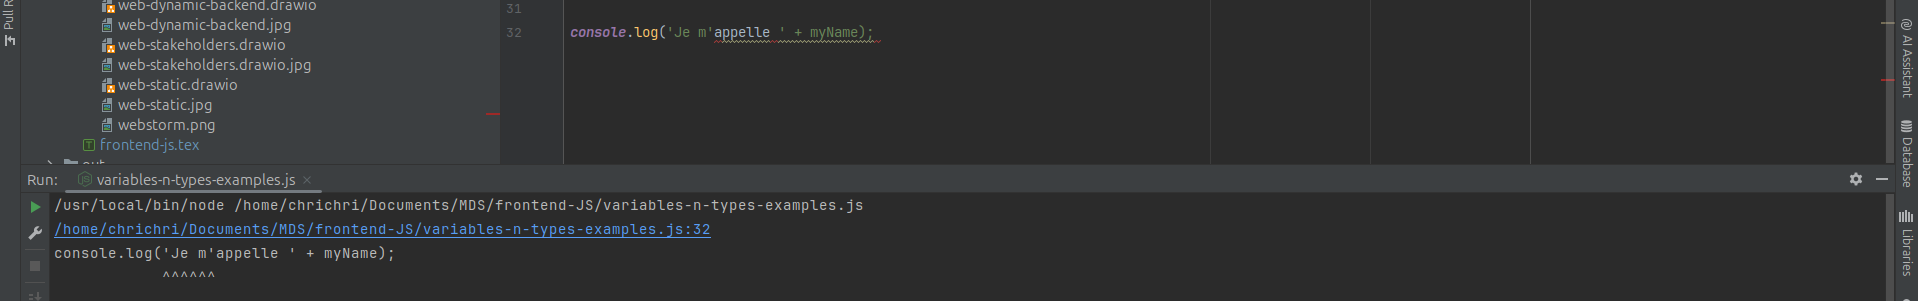
\includegraphics[width=12cm]{image/wrong-quote}
        \pause
        \bigbreak
        \flushleft
        Il faut des doubles quotes, mais on aurait pu s'en apercevoir avant, lors du développement, avec les avertissements en rouge dans l'IDE.
    \end{frame}

    \begin{frame}[fragile]{Déclarations et types}{Les booléens}
        \begin{footnotesize}
            \begin{itemize}
                \item En JavaScript, un booléen est un type de donnée qui ne peut avoir que deux valeurs~: \lstinline{true} (vrai) ou \lstinline{false} (faux).
                \item Les booléens sont souvent utilisés dans les structures de contrôle comme les conditions (\lstinline{if}, \lstinline{else}) et les boucles (\lstinline{while}, \lstinline{for}).
                \item Les expressions booléennes sont des expressions qui évaluent à \lstinline{true} ou \lstinline{false}.
                \item Les opérateurs de comparaison (comme \lstinline{==}, \lstinline{===}, \lstinline{!=}, \lstinline{!==}, \lstinline{>}, \lstinline{<}, \lstinline{>=}, \lstinline{<=}) et les opérateurs logiques (comme \lstinline{&&}, \lstinline{||}, \lstinline{!}) sont utilisés pour créer des expressions booléennes.
            \end{itemize}
        \end{footnotesize}
        \begin{lstlisting}[language=Bash]
> var isAdult = true;
undefined
> var isMinor = false;
undefined
>
> if (isAdult) {
...     console.log("Vous êtes un adulte.");
... } else {
...     console.log("Vous êtes un mineur.");
... }
Vous êtes un adulte.
        \end{lstlisting}
    \end{frame}

    \begin{frame}[fragile]{Déclarations et types}{Les booléens}
        Tester le contraire d'un booléan avec \lstinline{!}~:
        \begin{lstlisting}[language=Bash]
> var isAdult = true;
undefined
> var isMinor = false;
undefined
>
> if (!isMinor) {
...     console.log("Vous êtes un adulte.");
... } else {
...     console.log("Vous êtes un mineur.");
... }
Vous êtes un adulte.
        \end{lstlisting}
    \end{frame}

    \begin{frame}[fragile]{Déclarations et types}{Les booléens}
        Le booléen \lstinline{false} est un entier de valeur 0, tout le reste est \lstinline{true}.
        \bigbreak
        On peut le vérifier en explicitant le type avec \lstinline{Boolean}~:
        \begin{lstlisting}[language=Bash]
> var isAdult = Boolean(0);
undefined
> isAdult
false
> var isAdult = Boolean(1)
undefined
> isAdult
true
> var isAdult = Boolean(25)
undefined
> isAdult
        \end{lstlisting}
    \end{frame}

    \begin{frame}[fragile]{Déclarations et types}{Les valeurs vides}
        \begin{footnotesize}
            Il existe deux valeurs spéciales, écrites \lstinline{null} et \lstinline{undefined}, qui sont utilisées pour indiquer l'absence de valeur significative.
            Elles sont elles-mêmes des valeurs, mais elles ne contiennent aucune information.

            De nombreuses opérations dans le langage qui ne produisent pas de valeur significative renvoient \lstinline{undefined} simplement parce qu'elles doivent renvoyer une valeur.

            La différence de signification entre \lstinline{undefined} et \lstinline{null} est un accident de la conception de JavaScript, et cela n'a pas d'importance la plupart du temps.
            Dans les cas où vous devez réellement vous préoccuper de ces valeurs, je recommande de les traiter comme étant principalement interchangeables.
        \end{footnotesize}
        \begin{lstlisting}[language=Bash]
> var parkingLot;
undefined
> parkingLot
undefined
> var parkingLot2 = null;
undefined
> parkingLot == parkingLot2
true
        \end{lstlisting}
    \end{frame}

    \begin{frame}[fragile]{Déclarations et types}{Déclaration de manière explicite}
        Déclarer le type de manière explicite pour éviter des ambiguïtés~:
        \begin{lstlisting}[language=Bash]
> var t = String(9)
undefined
> t
'9'
> var t = Number("9")
undefined
> t
9
        \end{lstlisting}
        \begin{dangercolorbox}
            De manière générale, en programmation, il est considéré plus \textit{safe} d'être explicite.

            On dit souvent \textit{Explicit is better than implicit}.
        \end{dangercolorbox}
    \end{frame}

    \begin{frame}[fragile]{Déclarations et types}{Portée d'une variable\footnote{\label{label}\lstinline{let}, Mozilla, \url{https://developer.mozilla.org/fr/docs/Web/JavaScript/Reference/Statements/let}}}
        On peut déclarer une variable de deux manières~:
        \begin{itemize}
            \item Avec le mot clé \lstinline{var}, la variable est \textit{globale} ou \textit{fonctionnelle}.
            \item Avec le mot clé \lstinline{let}, la variable est défini pour un \textit{de bloc} délimité par les \lstinline[language=Javascript]!{ }! d'une boucle, condition, fonction, \textit{etc}.
        \end{itemize}
        \begin{lstlisting}[language=Bash]
> function x() {
...   y = 1; // Lève une exception ReferenceError en mode strict
...   var z = 2;
... }
undefined
> x();
undefined
> console.log(y); // Affiche "1" dans la console
1
undefined
> console.log(z); // Lève une exception ReferenceError car la portée est fonctionnelle:
Uncaught ReferenceError: z is not defined
        \end{lstlisting}
    \end{frame}

    \begin{frame}[fragile]{Déclarations et types}{Portée d'une variable\cref{label}}
        \begin{lstlisting}[language=Bash]
> let x = 1;
undefined
> if (x === 1) {
...   let x = 2;
...
...   console.log(x);
...   // Expected output: 2
... }
2
undefined
> console.log(x);
1
        \end{lstlisting}
        La modification de \lstinline{x} dans la condition n'a pas modifié le \lstinline{x} déclaré avant.
        \begin{dangercolorbox}
            Éviter d'utiliser \lstinline{var} pour déclarer des variables, préférer \lstinline{let} pour éviter les erreurs de portée.

            L'état d'une variable globale peut être difficile à analyser sur la totalité d'un programme.
        \end{dangercolorbox}
    \end{frame}

    \begin{frame}[fragile]{Déclarations et types}{Les constantes\footnote{\lstinline{const}, Mozilla, \url{https://developer.mozilla.org/fr/docs/Web/JavaScript/Reference/Statements/const}}}
        On peut déclarer une constante avec le mot clé \lstinline{const}.
        Par la suite, cette constante n'est accessible qu'en lecture.
        Une nouvelle valeur ne peut lui être affectée, une variable du même nom ne peut être à nouveau déclarée.
        \begin{lstlisting}[language=Bash,basicstyle=\tiny\ttfamily]
> const number = 42;
undefined
> try {
...   number = 99;
... } catch (err) {
...   console.log(err);
... }
TypeError: Assignment to constant variable.
    at REPL9:2:10
...
undefined
> console.log(number); // Pas de réassignation mais première valeur
42
        \end{lstlisting}
        \begin{dangercolorbox}
            Penser au fonctionnel de l'application et utiliser des \lstinline{const} dès que possible par sécurité, pour éviter des modifications non souhaitables.
        \end{dangercolorbox}
    \end{frame}

    \begin{frame}[fragile]{Déclarations et types}{Les étranges conversions automatiques de type}
        \begin{footnotesize}
            JavaScript est très flexible en ce qui concerne les types de données.
            Il convertit silencieusement de nombreux types de valeurs en d'autres types, pour que les choses fonctionnent comme prévu, c'est la \textit{type coercion}.
            Cela peut être pratique, mais parfois peu logique et donc peut aussi être source d'erreurs.
        \end{footnotesize}
        \begin{lstlisting}[language=Bash,basicstyle=\tiny\ttfamily]
> console.log(8 * null)
0
undefined
> console.log("5" - 1)
4
undefined
> console.log("5" + 1)
51
undefined
> console.log("five" * 2)
NaN
undefined
> console.log(false == 0)
true
undefined
> console.log(null == undefined);
true
undefined
> console.log(null == 0);
false
        \end{lstlisting}
    \end{frame}

    \subsection{Les opérateurs}\label{subsec:operators}
    \begin{frame}{Les opérateurs\footnote{\label{operators}Expressions et opérateurs, \url{https://developer.mozilla.org/fr/docs/Web/JavaScript/Guide/Expressions_and_operators}}}
        \begin{tiny}
            \begin{table}[h!]
                \centering
                \begin{tabular}{|c|c|p{8cm}|}
                    \hline
                    \textbf{Operator} & \textbf{Type} & \textbf{Description}             \\
                    \hline
                    +                 & Binary        & Addition or string concatenation \\
                    \hline
                    -                 & Binary        & Subtraction                      \\
                    \hline
                    *                 & Binary        & Multiplication                   \\
                    \hline
                    /                 & Binary        & Division                         \\
                    \hline
                    \%                & Binary        & Modulus (remainder)              \\
                    \hline
                    ++                & Unary         & Increment                        \\
                    \hline
                    --                & Unary         & Decrement                        \\
                    \hline
                    !                 & Unary         & Logical NOT                      \\
                    \hline
                    ==                & Binary        & Equality (abstract comparison)   \\
                    \hline
                    ===               & Binary        & Strict equality                  \\
                    \hline
                    !=                & Binary        & Inequality (abstract comparison) \\
                    \hline
                    !==               & Binary        & Strict inequality                \\
                    \hline
                    >                 & Binary        & Greater than                     \\
                    \hline
                    <                 & Binary        & Less than                        \\
                    \hline
                    >=                & Binary        & Greater than or equal to         \\
                    \hline
                    <=                & Binary        & Less than or equal to            \\
                    \hline
                    \&\&              & Binary        & Logical AND                      \\
                    \hline
                    ||                & Binary        & Logical OR                       \\
                    \hline
                    ?:                & Ternary       & Conditional (ternary) operator   \\
                    \hline
                    =                 & Binary        & Assignment                       \\
                    \hline
                    +=                & Binary        & Addition assignment              \\
                    \hline
                    -=                & Binary        & Subtraction assignment           \\
                    \hline
                    *=                & Binary        & Multiplication assignment        \\
                    \hline
                    /=                & Binary        & Division assignment              \\
                    \hline
                    \%=               & Binary        & Modulus assignment               \\
                    \hline
                \end{tabular}
            \end{table}
        \end{tiny}
    \end{frame}

    \begin{frame}{Les opérateurs}{Les opérateurs de comparaison\cref{operators}}
        \begin{tiny}
            \begin{table}[h!]
                \centering
                \begin{tabular}{|c|p{4cm}|c|}
                    \hline
                    \textbf{Opérateur}      & \textbf{Description}                                                                                                                     & \textbf{Exemple qui renvoie \lstinline{true}} \\
                    \hline
                    Égalité (==)            & Renvoie \lstinline{true} si les opérandes sont égaux (après conversion implicite). & \lstinline{3 == '3'}   \\
                    \hline
                    Inégalité (!=)          & Renvoie \lstinline{true} si les opérandes sont différents (après conversion implicite). & \lstinline{var2 != "3"} \\
                    \hline
                    Égalité stricte (===)   & Renvoie \lstinline{true} si les opérandes sont égaux et du même type. Voir également \lstinline{Object.is()} et l'égalité en JavaScript. & \lstinline{3 === var1} \\
                    \hline
                    Inégalité stricte (!==) & Renvoie \lstinline{true} si les opérandes sont du même type et différents ou s'ils ne sont pas du même type.  & \lstinline{3 !== '3'}        \\
                    \hline
                    Supériorité stricte (>) & Renvoie \lstinline{true} si l'opérande gauche est strictement supérieur à l'opérande droit.                   & \lstinline{'12' > 2}        \\
                    \hline
                    Supériorité (>=)        & Renvoie \lstinline{true} si l'opérande gauche est supérieur ou égal à l'opérande droit.                       & \lstinline{var1 >= 3}        \\
                    \hline
                    Infériorité stricte (<) & Renvoie \lstinline{true} si l'opérande gauche est strictement inférieur à l'opérande droit.                   & \lstinline[language=Javascript]!"2" < 12!        \\
                    \hline
                    Infériorité (<=)        & Renvoie \lstinline{true} si l'opérande gauche est inférieur ou égal à l'opérande droit.                       & \lstinline{var2 <= 5}        \\
                    \hline
                \end{tabular}
            \end{table}
        \end{tiny}
    \end{frame}

    \begin{frame}{Les opérateurs}{Les opérateurs de comparaison\cref{operators}}
        Exercice \execcounterdispinc{}~:
        \begin{itemize}
            \item Quand on compare des chaines de caractères, quel est l'ordre des caractères alphanumériques (lettres et chiffres)~?
            \item Comparer \lstinline{null} avec \lstinline{0} et aussi \lstinline{Infinity}. Est-ce logique~?
            \item Comparer \lstinline{null} avec \lstinline{undefined}. Est-ce logique~?
        \end{itemize}
        \bigbreak
        \centering
        
\includegraphics[width=3cm]{image/intelligence}
    \end{frame}

    \begin{frame}{Les opérateurs}{Les opérateurs arithmétiques\cref{operators}}
        \begin{tiny}
            \begin{table}[h!]
                \centering
                \begin{tabular}{|c|p{4cm}|p{4cm}|}
                    \hline
                    \textbf{Opérateur}              & \textbf{Description}                                                                                                                                                                                                                                                                      & \textbf{Exemple}                                                                                                                                                                                                                                 \\
                    \hline
                    Reste (\%)                      & Un opérateur binaire qui renvoie le reste entier de la division des deux opérandes. & \lstinline{12 \% 5} renvoie \lstinline{2}. \\
                    \hline
                    Incrément (++)                  & Un opérateur unaire qui ajoute un à son opérande. S'il est utilisé en opérateur préfixe (\lstinline{++x}), il renvoie la valeur de son opérande après y avoir ajouté un. S'il est utilisé en opérateur suffixé (\lstinline{x++}), il renvoie la valeur de l'opérande avant l'ajout de un. & Si \lstinline{x} vaut 3, alors \lstinline{++x} définit \lstinline{x} avec \lstinline{4} et renvoie \lstinline{4}, tandis que \lstinline{x++} renvoie \lstinline{3} puis, uniquement après, définit \lstinline{x} avec \lstinline{4}. \\
                    \hline
                    Décrément (--)                  & Un opérateur unaire qui soustrait un à son opérande. La valeur de retour est analogue à celle de l'opérateur d'incrément. & Si \lstinline{x} vaut \lstinline{3}, alors \lstinline{--x} définit \lstinline{x} avec \lstinline{2} et renvoie \lstinline{2}, tandis que \lstinline{x--} renvoie \lstinline{3} puis, uniquement après, définit \lstinline{x} avec \lstinline{2}. \\
                    \hline
                    Négation unaire (-)             & Un opérateur unaire qui renvoie l'opposé de l'opérande.                                                                                                                                                                                                                                   & Si \lstinline{x} vaut 3, \lstinline{-x} renvoie \lstinline{-3}.                                                                                                                                                                                  \\
                    \hline
                    Plus unaire (+)                 & Un opérateur unaire qui tente la conversion de l'opérande en nombre si ce n'est pas déjà une valeur numérique. & \lstinline{+"3"} renvoie \lstinline{3}. \newline \lstinline{+true} renvoie \lstinline{1}. \\
                    \hline
                    Opérateur d'exponentiation (**) & Élève une base donnée par l'opérande gauche à la puissance donnée par l'opérande droit. & \lstinline{2 ** 3} renvoie \lstinline{8}. \newline \lstinline{10 ** -1} renvoie \lstinline{0.1}. \\
                    \hline
                \end{tabular}
            \end{table}
        \end{tiny}
    \end{frame}

    \begin{frame}{Les opérateurs}{Les opérateurs arithmétiques\cref{operators}}
        Exercice \execcounterdispinc{}~:
        \begin{itemize}
            \item Quelle est la différence entre \lstinline{++x} et \lstinline{x++}~?
            \item Quelle est la différence entre \lstinline{Infinity} et \lstinline{Infinity}~?
            \item Quelle est la différence entre \lstinline{null} et \lstinline{undefined}~?
            Est-ce logique par rapport à ce que nous avons vu précédemment avec les opérateurs de comparaison~?
            \item Additionner deux chaines de caractères.
            \item Soustraire deux chaines de caractères.
            Étonnant non~?
            \item Utiliser \lstinline{\%} pour vérifier si un nombre est pair ou impair.
        \end{itemize}
        \bigbreak
        \centering
        
\includegraphics[width=3cm]{image/intelligence}
    \end{frame}

    \begin{frame}{Les opérateurs}{Opérateurs logiques\cref{operators}}
        \begin{scriptsize}
            Les plus utilisés...
            \begin{table}[h!]
                \centering
                \begin{tabular}{|c|c|p{7cm}|}
                    \hline
                    \textbf{Opérateur}          & \textbf{Utilisation}         & \textbf{Description}                                                                                                                                                                                                                                                                                                 \\
                    \hline
                    ET logique \lstinline{\&\&} & \lstinline{expr1 \&\& expr2} & Renvoie \lstinline{expr1} si elle peut être convertie en \lstinline{false} et renvoie \lstinline{expr2} sinon. Lorsqu'il est utilisé avec des valeurs booléennes, \lstinline{\&\&} renvoie \lstinline{true} si les deux opérandes valent \lstinline{true} et \lstinline{false} sinon.                                \\
                    \hline
                    OU logique \lstinline{||}   & \lstinline{expr1 || expr2}   & Renvoie \lstinline{expr1} si elle peut être convertie en \lstinline{true} et renvoie \lstinline{expr2} sinon. Lorsqu'il est utilisé avec des valeurs booléennes, \lstinline{||} renvoie \lstinline{true} si l'un des deux opérandes vaut \lstinline{true} et \lstinline{false} si les deux valent \lstinline{false}. \\
                    \hline
                    NON logique \lstinline{!}   & \lstinline{!expr}            & Renvoie \lstinline{false} si son unique opérande peut être converti en \lstinline{true}, renvoie \lstinline{true} sinon.                                                                                                                                                                                             \\
                    \hline
                \end{tabular}
            \end{table}
            \begin{dangercolorbox}
                Ne pas confondre \lstinline{||} et \lstinline{|}, \lstinline{\&\&} et \lstinline{\&}.
                Les logiques, comme ici, évaluent le membre différent de \lstinline{0} si l'expression est \lstinline{true}.
            \end{dangercolorbox}
        \end{scriptsize}
    \end{frame}

    \begin{frame}[fragile]{Les opérateurs}{Opérateur conditionnel A.K.A. ternaire}
        \begin{small}
            L'opérateur conditionnel est le seul opérateur JavaScript à prendre trois opérandes. Il permet d'affecter une valeur ou en une autre selon une condition donnée. Sa syntaxe est la suivante :
            \begin{lstlisting}[language=JavaScript]
condition ? val1 : val2;
            \end{lstlisting}
            Si la condition est vraie, l'expression sera résolue avec la valeur de \lstinline{val1}.
            Sinon, elle sera résolue avec la valeur de \lstinline{val2}.
            L'opérateur conditionnel peut être utilisé à tout endroit où un opérateur standard peut être utilisé.
            \bigbreak
            Par exemple :
            \begin{lstlisting}[language=Bash]
> let age = 19;
undefined
> const statut = age >= 18 ? "adulte" : "mineur";
undefined
> statut
'adulte'
            \end{lstlisting}
            Cette instruction affecte la valeur \lstinline{"adulte"} à la variable \lstinline{statut} si \lstinline{age} est supérieur ou égal à 18. Sinon, c'est la valeur \lstinline{"mineur"} qui est affectée à \lstinline{statut}.
        \end{small}
    \end{frame}

    \begin{frame}{Les opérateurs}{Opérateur conditionnel A.K.A. ternaire}
        Exercice \execcounterdispinc{}~:
        \begin{itemize}
            \item Stocker un booléen dans \lstinline{major} si la variable \lstinline{age} est supérieur à 18.
            \item Stocker la chaine de caractère \lstinline{pair} dans la variable \lstinline{pairOrImpair} si \lstinline{x} est pair, sinon stocker la chaine de caractère \lstinline{impair}.
            \item Stocker un booléen dans \lstinline{pairBool} si \lstinline{x} est pair.
        \end{itemize}
        \bigbreak
        \centering
        
\includegraphics[width=3cm]{image/intelligence}
    \end{frame}

    \begin{frame}{Les opérateurs}{Opérateurs binaires\cref{operators}}
        \begin{scriptsize}
            Pas les plus utilisés...
            \begin{table}[h!]
                \centering
                \begin{tabular}{|p{3cm}|c|p{6cm}|}
                    \hline
                    \textbf{Opérateur}                                 & \textbf{Utilisation}                     & \textbf{Description}                                                                                                                                            \\
                    \hline
                    ET binaire                                         & \lstinline{a \& b}                       & Renvoie \lstinline{1} à chaque position pour laquelle les bits des deux opérandes valent \lstinline{1}.                                                         \\
                    \hline
                    OU binaire                                         & \lstinline{a | b}                        & Renvoie \lstinline{0} à chaque position pour laquelle les bits des deux opérandes valent \lstinline{0}.                                                         \\
                    \hline
                    OU exclusif binaire                                & \lstinline{a \^ b}                       & Renvoie \lstinline{0} à chaque position pour laquelle les bits sont les mêmes. Renvoie \lstinline{1} à chaque position où les bits sont différents.             \\
                    \hline
                    NON binaire                                        & \lstinline{\~a}                          & Inverse les bits de l'opérande.                                                                                                                                 \\
                    \hline
                    Décalage à gauche                                  & \lstinline[language=Javascript]! a << b! & Décale la représentation binaire de \lstinline{a} de \lstinline{b} bits vers la gauche, en ajoutant des \lstinline{0} à droite.                                 \\
                    \hline
                    Décalage à droite avec propagation du signe        & \lstinline[language=Javascript]!a >> b!  & Décale la représentation binaire de \lstinline{a} de \lstinline{b} bits vers la droite, en enlevant les bits en trop.                                                       \\
                    \hline
                    Décalage à droite avec remplissage à \lstinline{0} & \lstinline[language=Javascript]!a >>> b! & Décale la représentation binaire de \lstinline{a} de \lstinline{b} bits vers la droite, en enlevant les bits en trop et en ajoutant des \lstinline{0} à gauche.             \\
                    \hline
                \end{tabular}
            \end{table}
            \begin{dangercolorbox}
                Ne pas confondre \lstinline{||} et \lstinline{|}, \lstinline{\&\&} et \lstinline{\&}.
                Les binaires comme ici, renvoient toujours \lstinline{0} ou \lstinline{1}, les autres, les logiques évaluent le membre différent de \lstinline{0}.
            \end{dangercolorbox}
        \end{scriptsize}
    \end{frame}

    \begin{frame}{Les opérateurs}{Opérateurs binaires\cref{operators}}
        Certaines anciennes machines et programmes utilisaient les opérateurs binaires pour accélérer l'arithmétique.
        Par exemple le décalage à gauche \lstinline[language=Javascript]! a << b! est équivalent à \lstinline{a * 2^b}.
        Le décalage à droite \lstinline[language=Javascript]! a >> b! est équivalent à \lstinline{a / 2^b}.
        \bigbreak
        Exercice \execcounterdispinc{}~:
        \begin{itemize}
            \item Stocker dans la variable \lstinline{multBySixtyFour} l'entier égal à \lstinline{8 * 64} en utilisant un opérateur binaire.
            \item Stocker dans la variable \lstinline{divBySixtyFour} l'entier égal à \lstinline{512 / 32} en utilisant un opérateur binaire.
            \item Vérifier que \lstinline{x \&1} permet de vérifier que \lstinline{x} est impair.
            \item À partir de l'expression \lstinline{x \&1} quel opérateur peut-on utiliser pour vérifier que est pair~?
            \item Stocker un booléen dans \lstinline{pairBool} si \lstinline{x} est pair à l'aide de l'opérateur \lstinline{\&} et de la déclaration de type \lstinline{Boolean}.
        \end{itemize}
    \end{frame}

    \subsection{Les fonctions}\label{subsec:functions}
    \begin{frame}[fragile]{Les fonctions}{Déclarations\footnote{\label{mozilla-function}Définir des fonctions, Mozilla, \url{https://developer.mozilla.org/fr/docs/Web/JavaScript/Guide/Functions}}}
        Une définition de fonction (aussi appelée déclaration de fonction ou instruction de fonction) est construite avec le mot-clé \href{https://developer.mozilla.org/fr/docs/Web/JavaScript/Reference/Statements/function}{function}, suivi par :
        \begin{itemize}
            \item L'éventuel nom de la fonction, sinon c'est une fonction anonyme.
            \item Une \textbf{éventuelle} liste d'arguments à passer à la fonction, entre parenthèses et séparés par des virgules.
            \item Les instructions JavaScript définissant la fonction, entre accolades, \lstinline[language=Javascript]!\{ \}!.
            \item L'\textbf{éventuel} instruction \lstinline{return} si la fonction doit renvoyer une valeur, un objet, \textit{etc}.
        \end{itemize}
        \bigbreak
        Le code suivant, par exemple, définit une fonction intitulée square~:
        \begin{lstlisting}[language=JavaScript]
function square(number) {
    return number * number;
}
        \end{lstlisting}
    \end{frame}

    \begin{frame}[fragile]{Les fonctions}{Déclarations\cref{mozilla-function}}
        La fonction square prend un seul argument, appelé number.
        La fonction est composée d'une seule instruction qui renvoie l'argument de la fonction (number) multiplié par lui-même.
        L'instruction \href{https://developer.mozilla.org/fr/docs/Web/JavaScript/Reference/Statements/return}{return} spécifie la valeur qui est renvoyée par la fonction.~:
        \begin{lstlisting}[language=JavaScript]
    return number * number;
        \end{lstlisting}
        \begin{dangercolorbox}
            Les paramètres primitifs (comme les nombres) sont passés à la fonction par valeur.
            La valeur est passée à la fonction mais si cette dernière change la valeur du paramètre, cela n'aura pas d'impact au niveau global ou au niveau de ce qui a appelé la fonction.
        \end{dangercolorbox}
        Qu'est-ce que ça veut dire~?
    \end{frame}

    \begin{frame}{Les fonctions}{Les caractéristiques et bonnes pratiques}
        \begin{itemize}
            \item Elles sont courtes, sont atomiques et font une seule chose.
            Mieux vaut les imbriquer que d'avoir une grosse fonction complexe.
            \item Elles sont nommées de manière explicite, avec un verbe décrivant leur action.
            \item Leurs commentaires sont simples car elles sont simples.
            \item Peuvent appeler d'autres fonctions ou s'appeler elle-même (fonction récursive).
            \item On les sépare en 2 familles~:
            \begin{itemize}
                \item Les fonctions \textit{pures}, qui appliquent une transformation sur des données passées en argument et renvoient un résultat.
                Sans aucune action sur le environnement.
                \item Les fonctions \textit{avec effet de bord}, qui modifient l'environnement.
                Appel d'API, log dans la console, \textit{etc}.
            \end{itemize}
        \end{itemize}
    \end{frame}

    \begin{frame}[fragile]{Les fonctions}{Appeler une fonction\cref{mozilla-function}}
        Une fois que la fonction est définie, elle peut être appelée par son nom suivi de parenthèses et des arguments à passer à la fonction entre ces parenthèses.
        Par exemple, pour appeler la fonction carré définie précédemment.
        Par convention on termine l'appel par \lstinline{;}.
        Si la fonction a un \lstinline{return}, la valeur retournée peut être stockée dans une variables~:
        \begin{lstlisting}[language=Bash]
> function square(nombre) {
...     return nombre * nombre;
... }
undefined
> let twoSquared = square(2);
undefined
> twoSquared
4
> square(2);
4
        \end{lstlisting}
    \end{frame}

    \begin{frame}[fragile]{Les fonctions}{La portée de la fonction\cref{mozilla-function}}
        Il est possible d'imbriquer une fonction au sein d'une fonction.
        La fonction imbriquée (interne) est privée par rapport à la fonction (externe) qui la contient. Cela forme ce qu'on appelle une fermeture (\textit{closure} en anglais).
        \begin{lstlisting}[language=Bash]
> function ajouteCarres(a, b) {
...   function carre(x) {
...     return x * x;
...   }
...   return carre(a) + carre(b);
... }
undefined
> let a = ajouteCarres(2, 3); // renvoie 13
undefined
> let b = ajouteCarres(3, 4); // renvoie 25
undefined
> let c = ajouteCarres(4, 5); // renvoie 41
        \end{lstlisting}
    \end{frame}

    \begin{frame}[fragile]{Les fonctions}{La portée de la fonction\cref{mozilla-function}}
        \begin{tiny}
            Une fermeture est une expression (généralement une fonction) possédant des variables libres ainsi qu'un environnement qui lie ces variables (autrement dit qui \textit{ferme} l'expression).
            \bigbreak
            Étant donné qu'une fonction imbriquée est une fermeture, cela signifie que la fonction imbriquée peut \textit{hériter} des arguments et des variables de la fonction qui la contient.
            En d'autres termes, la fonction interne contient la portée de la fonction externe.
            \bigbreak
            Pour résumer :
            \begin{itemize}
                \item On ne peut accéder à la fonction interne seulement avec des instructions contenues dans la fonction externe.
                \item La fonction interne est une fermeture~: la fonction interne peut utiliser des arguments et des variables de la fonction externe alors que la fonction externe ne peut pas utiliser de variables et d'arguments de la fonction interne.
            \end{itemize}
        \end{tiny}
        \begin{lstlisting}[language=Bash,basicstyle=\tiny\ttfamily]
function externe(x) {
  function interne(y) {
    return x + y;
  }
  return interne;
}
let fn_interne = externe(3);
let resultat = fn_interne(5); // renvoie 8

let resultat1 = externe(3)(5); // renvoie 8
undefined
> resultat
8
> resultat1
8
        \end{lstlisting}
    \end{frame}

    \begin{frame}{Les fonctions}{Exercice \execcounterdispinc{}}
        \begin{itemize}
            \item Développer une fonction récursive appelé \lstinline{factorial} qui prend en entrée un entier et calcul le factoriel.
            C'est donc une fonction pure.
            \item Appeler la fonction et trouver à quel nombre le factoriel est assimilé à \lstinline{Infinity}.
            \item Développer une seconde fonction avec effet de bord seulement, appelée \lstinline{displayFactorialResult}, qui affiche le résultat dans la console avec les fonctions \lstinline{console.log} et \lstinline{factorial}.
            Le message doit être~: \lstinline{"Le factoriel de 5 est 120."}.
        \end{itemize}
        \bigbreak
        \centering
        
\includegraphics[width=3cm]{image/intelligence}
    \end{frame}

    \begin{frame}[fragile]{Les fonctions}{Les \textit{arrows functions}}
        La dernière norme ES6 a introduit les \textit{arrows functions} ou fonctions fléchées en bon français.
        Leur syntaxe est plus courte et parfois donc plus lisible.
        Elles peuvent aussi être anonymes.

        Cette syntaxe s'inspire de la programmation fonctionnelle et des fonctions \textit{lambda}.
        \begin{dangercolorbox}
            Les fonctions fléchées ne sont pas adaptées à tous les usages, il faut les réserver aux fonctions pures et simples.
        \end{dangercolorbox}
        La syntaxe est la suivante~:
        \begin{lstlisting}[language=JavaScript]
function squareOldStyle(nombre) {
    return nombre * nombre;
}
const squareArrowStyle = (nombre) => nombre * nombre;
        \end{lstlisting}
        \begin{dangercolorbox}
            Le \lstinline{return} est implicite~!
        \end{dangercolorbox}
    \end{frame}

    \begin{frame}{Les fonctions}{Exercice \execcounterdispinc{}}
        Que font ces packages JS en lignes~?
        \begin{itemize}
            \item \url{https://www.npmjs.com/package/is-odd}
            \item \url{https://www.npmjs.com/package/is-even}
            \item \url{https://www.npmjs.com/package/is-odd-ai}
            \item \url{https://www.npmjs.com/package/is-even-ai}
        \end{itemize}
        Est-ce utile?
        \bigbreak
        Est-ce dangereux~?
        \bigbreak
        \centering
        
\includegraphics[width=3cm]{image/intelligence}
    \end{frame}

    \begin{frame}{Les fonctions}{Exercice \execcounterdispinc{}}
        Développer les mêmes fonctions avec des fonctions fléchées en un minimum de caractères/ligne de code possible (Moins de code = moins de bugs \emoji{wink}).
        \bigbreak
        \begin{itemize}
            \item La fonction \lstinline{isOdd} qui renvoie \lstinline{true} si le nombre est impair.
            \item La fonction \lstinline{isEven} qui renvoie \lstinline{true} si le nombre est pair.
            \item Développer une fonction à partir de l'autre.
        \end{itemize}
        \bigbreak
        \centering
        
\includegraphics[width=3cm]{image/intelligence}
    \end{frame}


    \section{Licence CC}\label{sec:licence}

    \begin{frame}{Licence}{Licence Creative Commons}
        Support de cours sous licence Creative Commons BY-NC-ND~.
        \bigbreak
        Vous pouvez donc, partager, copier, distribuer le document.
        \bigbreak
        Attribution requise à PapIT SASU - Pas d’utilisation commerciale - Pas de modification
        \bigbreak
        \centering
        
\includegraphics[width=5cm]{image/by-nc-nd-logo}
    \end{frame}


\end{document}
